\documentclass[10pt]{article}
\usepackage[a4paper,margin=1.60cm]{geometry}
\usepackage[T1]{fontenc}
\usepackage[english,french]{babel}
\frenchsetup{SmallCapsFigTabCaptions=false}
\addto\captionsfrench{\renewcommand{\tablename}{Tableau}}
\usepackage{lmodern}
\usepackage{microtype}
\usepackage{graphicx}
\usepackage{booktabs}
\usepackage{tabularx}
\usepackage{array}
\usepackage{amsmath,amssymb}
\usepackage{xcolor}
\usepackage[hidelinks]{hyperref}
\usepackage{caption}
\captionsetup{font=small,labelfont=bf}
\setlength{\parskip}{3.2pt}
\graphicspath{{../research/timecourse/figures/}{../research/revision/figures/}{../research/study09/figures/}{../research/study10/figures/}}
\newcolumntype{L}[1]{>{\raggedright\arraybackslash}p{#1}}
\newcolumntype{Y}{>{\raggedright\arraybackslash}X}

\title{Neurophysiologie, prévision cerveau--cœur, limites de généralisation et monitoring passif du stress aigu chez 314 personnes\\
\large Synthèse complète des Études 04 à 10 sur le jeu de données HABS}
\author{Équipe 12 : Mathias Chebbah, Aurélien Saint-Grégoire, Ashley Russo\\
\small HABS Neuro-AI Hackathon, Université Paris-Saclay, novembre 2026}
\date{}

\begin{document}
\maketitle

\begin{abstract}
\noindent Lors d'une exposition brève (10~s) à un stimulus audiovisuel aversif, que révèlent réellement l'électroencéphalogramme (EEG 64 voies) et les signaux périphériques (ECG, conductance cutanée EDA, respiration, oculométrie) chez l'humain, dans quelle mesure l'EEG précoce anticipe-t-il la réponse autonome future au-delà du passé corporel, et quelles performances opérationnelles un détecteur multimodal sans fuite atteint-il en vue d'un monitoring clinique non verbal ? Nous présentons la synthèse intégrée de sept campagnes pré-enregistrées (Études~04 à~10) menées sur le jeu de données HABS (314 adultes sains, 22\,974 essais valides, 508 enregistrements, 252 clips audiovisuels de 10~s répartis en 84 thèmes et 5 cohortes), appuyée sur une revue critique de 39 publications de référence et une comptabilité reproductible totale (3,70~H100-h GPU, $\approx 4{,}0$~CPU-h pour les audits finaux).

Sept résultats majeurs structurent notre contribution. \textbf{(1)~Architecture tri-branche du stress aigu bref.} Le critère de stress ($V \le 4$ et $A \ge 6$) regroupe 89,2\,\% d'émotions négatives en premier choix (97,2\,\% sur les trois choix ; optimum de détection à $3/7$). Les réponses suivent une cascade fixe (EEG delta $<1$~s $\to$ freinage cardiaque et respiration 1--2~s $\to$ EDA 4--10~s) articulant trois branches : désynchronisation alpha occipitale automatique ($d = -0{,}33$ à $-0{,}41$ même chez les spectateurs calmes), freinage vagal sinusal évaluatif (allongement RR $+5{,}06$~ms, segment PR nul $-0{,}05$~ms, artefact QTc de Bazett annulé après $\Delta\mathrm{RR}$, absent chez les spectateurs calmes devant des vidéos stressantes : $-0{,}49$ vs $-3{,}08$~bpm ; apparié $-2{,}97$~bpm, $d = -0{,}41$, AUC vidéo fixe $0{,}525 \to 0{,}564$), et alarme sympathique/corticale à seuil élevé ($A \ge 7$ : doublement de l'EDA et du delta centro-pariétal, résistant à 93\,\% à un contrôle oculaire pré-ICA ; potentiel évoqué cardiaque nul avec ou sans ICA, $+0{,}038$ vs $+0{,}039$). En dynamique intra-clip ($N = 209$), la peur et le dégoût divergent nettement : le dégoût domine le delta précoce ($-0{,}098$) et le gamma frontal tardif ($-0{,}178$, prudence micro-EMG), tandis que la peur domine la suppression alpha ($-0{,}137$), la bradycardie tardive et l'explosion électrodermale tardive ($+0{,}193$, transition $+0{,}303$). \textbf{(2)~Audit des fuites et prévision causale EEG $\to$ Cœur.} Corriger le centrage transductif par sujet ($+0{,}0141$ en LogReg) et l'attention bidirectionnelle de \texttt{REVE-base} couplée aux thèmes vus ($+0{,}059$ ECG, $+0{,}069$ Resp) révèle, sous mur causal strict à $t = 5{,}000$~s en \emph{cold-start} (\texttt{dev} $3\times 3$), un gain prédictif cardiaque réel, modeste, résistant aux artefacts et strictement idiosyncrasique : $\Delta r = +0{,}0089$ résiduel, $+0{,}0110$ conjoint (71,4\,\% améliorés, $q_{\text{FDR}} < 10^{-6}$), $+0{,}0063$ au-dessus de \texttt{M0\_gbdt}, $+0{,}0182$ sur l'incrément pur $\Delta\mathrm{FC}$, persistant à 2~s ($+0{,}0089$) et 5~s ($+0{,}0038$) de garde, nul en permutation intra-sujet ($-0{,}0003$) et en pré-stimulus ($-0{,}0010$), détruit si l'on substitue l'EEG d'un autre spectateur de la même vidéo ($+0{,}0242$, intra-vidéo $+0{,}0065$), et \textbf{répliqué dans 5/5 cohortes en transfert hors-cohorte LOCO} ($+0{,}0107$ [$+0{,}0071 ; +0{,}0145$], 68,8\,\%). La même hypothèse est strictement réfutée sur l'EDA ($-0{,}0097$) et la respiration ($+0{,}0008$, \texttt{M0\_gbdt} $= 0{,}7036$). \textbf{(3)~Modèles fondation EEG, SSL et factorisation Trait/État.} Sur le stress subjectif double-inédit, aucun modèle fondation (\texttt{REVE}, \texttt{LaBraM}, \texttt{CBraMod}, \texttt{EEGPT}, \texttt{Signal-JEPA}), ni \texttt{PhysioJEPA}, ni l'adaptation LoRA ($-0{,}0069$ pour $21{,}7\times$ plus de GPU), ni le stacking OOF ne dépassent les 4 phases linéaires enrichies (0 GPU : AUC $0{,}569$ en \texttt{dev} Cold-Start, $0{,}586$--$0{,}589$ sur test scellé), alors que la perte de ranking intra-sujet est décisive ($+0{,}0406$) et que le \emph{shrinkage} bayésien empirique abaisse la variance d'identité ($51\,\% \to 37\,\%$) tout en améliorant la calibration. \textbf{(4)~Échelle de généralisation et ablation.} Passer d'un split aléatoire (R1 : $0{,}589$) au double inédit Cold-Start (R4 : $0{,}569$) révèle 70\,\% d'inflation par thèmes vus et $+0{,}041$ d'inflation biométrique poolée sur \texttt{REVE} ; en R4, l'EEG ($-0{,}028^*$) et l'EDA ($-0{,}018^*$) forment les deux piliers complémentaires (ECG isolé $0{,}508$). \textbf{(5)~Stabilité longitudinale J1 $\to$ J2 et habituation.} L'EDA présente la plus faible stabilité tonique ($r = 0{,}420$) et son décodeur chute significativement d'un jour à l'autre ($0{,}560 \to 0{,}523$, $-0{,}039^*$), comme la respiration ($-0{,}030^*$), tandis que l'EEG et le multimodal tiennent ; les pics SCR s'habituent ($-0{,}032^*$), pas le cœur vagal ni l'alpha. \textbf{(6)~Personnalisation $k$-shot et CORAL.} La personnalisation supervisée naïve s'effondre massivement jusqu'à $k = 40$ ($-0{,}081$ à $-0{,}053$) et sur J1 $\to$ J2 ($-0{,}040^*$ à $-0{,}069^*$) ; le \emph{shrinkage} bayésien MAP supprime la chute sans franchir de saut majeur ; CORAL reste neutre en LOCO ($0{,}589 \to 0{,}588$). \textbf{(7)~Cohérence autonome--subjective et monitoring clinique passif.} Sur $N = 314$ ($n = 16\,276$), l'espace affectif se décompose en trois facteurs orthogonaux (EDA, neuro-cardio autonome décorrélé du ressenti, et axe subjectif--cardio-respiratoire) ; 79\,\% des individus sont cohérents en composite (21\,\% discordants ; effet d'intensité $+0{,}101^*$). Agréger 10 épisodes passifs (100~s) en Cold-Start porte l'AUC à $0{,}680$--$0{,}698$ et double la sensibilité à 90\,\% de spécificité (jusqu'à 53\,\%), fixant des bornes quantitatives lucides pour la clinique non verbale.
\end{abstract}

\section{Introduction : neurophysiologie du stress aigu et défi du monitoring non verbal}

Évaluer objectivement une réaction de stress aigu ou de détresse sans recours à l'auto-évaluation verbale représente un verrou majeur à l'intersection des neurosciences affectives, de l'apprentissage automatique et de la médecine clinique. Chez un nouveau-né exposé à une procédure douloureuse \cite{roue2025}, un patient en \emph{locked-in syndrome} \cite{adama2025}, un patient présentant un trouble de la conscience \cite{engemann2018,candia2021} ou un patient sous anesthésie générale et soins critiques \cite{danel2025}, aucune échelle verbale n'est disponible. Or un biomarqueur clinique utile ne peut se contenter de détecter un réflexe sensoriel déclenché par un stimulus saillant : il doit refléter une réactivité émotionnelle ou nociceptive réellement vécue, généraliser à des individus et des contextes jamais rencontrés, résister aux dérives temporelles entre sessions et rester honnêtement calibré face à l'hétérogénéité inter-individuelle \cite{paniagua2025}.

Une revue systématique de 39 publications récentes et fondatrices structure cet enjeu autour de cinq axes qui soulèvent autant de questions empiriques ouvertes sur grande cohorte :
\begin{enumerate}
\item \textbf{Dissociation autonome sur fenêtres courtes (5--10~s).} Le système nerveux autonome (SNA) n'agit pas comme un bloc monolithique \cite{jennings1980,collet1997}. Face à des stimuli affectifs brefs, la décélération cardiaque rapide est médiée par un freinage vagal sur le nœud sino-atrial \cite{somsen2002,abercrombie2008,palomba2000,hagenaars2014}, distinct cinétiquement et fonctionnellement de la sudation sympathique électrodermale (SCR) qui survient plus tard et présente une habituation propre \cite{chen2014,benedek2010}. La variabilité cardiaque ultra-courte (RMSSD sur $\le 30$~s) échoue à séparer la valence et reflète surtout l'orientation visuelle \cite{schippers2018,munoz2015}, tandis que les profils autonomes diffèrent d'une émotion négative à l'autre \cite{qin2023,siegel2018}, plaidant pour une approche multimodale combinant ECG, EDA et respiration \cite{coelli2026}. De plus, les relations physiologie--arousal dérivent dans le temps, l'EDA fluctuant bien plus que la fréquence cardiaque d'une session à l'autre \cite{sakimura2025}.
\item \textbf{Décalage temporel EEG/SNA et pièges de généralisation.} L'EEG capture une évaluation affective sémantique et attentionnelle en quelques centaines de millisecondes \cite{jeong2026,jomaa2026,alasfour2025}, bien avant les effecteurs autonomes périphériques ; à l'intérieur même d'un extrait vidéo, la peur et le dégoût mobilisent des bandes spectrales distinctes au fil du temps \cite{si2026}. Parallèlement, la littérature d'apprentissage automatique multimodal \cite{liu2021} montre que les découpages aléatoires gonflent massivement les scores par rapport à une validation stricte inter-sujets (LOSO) et inter-stimuli \cite{alshamrani2026,hinduja2023,gerster2026,li2026}, tandis que des méthodes d'adaptation de domaine sans étiquette comme CORAL \cite{sun2016,mihirette2025} sont proposées pour compenser les décalages de contexte, là où la généralisation EEG inter-centres est démontrée sur les états de conscience (AUC $0{,}73$--$0{,}78$ \cite{engemann2018}).
\item \textbf{EEG, attention visuelle et déploiement inter-sujets.} Sur images et clips vidéo émotionnels, la désynchronisation alpha occipito-pariétale (8--13~Hz) assure un filtrage sensoriel (\emph{gating}) et signale l'engagement attentionnel soutenu ou l'immobilité vigilante face à une menace \cite{zumer2014,panitz2019,bacigalupo2022,codispoti2023,stegmann2024}, avec une modulation distincte en vidéo dynamique par rapport aux images fixes \cite{simons2009,kim2021,romeo2022}. Toutefois, les études diagnostiques de déploiement inter-sujets soulignent la fragilité de la classification EEG brute due à l'ambiguïté des auto-évaluations \cite{lifan2024} et alertent qu'une personnalisation supervisée avec moins de 20 essais labellisés par individu peut être contre-productive \cite{khan2026}.
\item \textbf{Évaluation subjective, cohérence autonome et différences trait vs état.} La correspondance intra-individuelle entre expérience subjective et réponses autonomes varie fortement d'un individu à l'autre et se renforce aux hautes intensités \cite{brown2019,sato2020,mauss2005}. L'analyse de l'espace affectif autonome--subjectif montre une dimension de cohérence partagée distincte d'une dimension purement autonome orthogonale au ressenti \cite{cuve2023}, modulée par les traits de personnalité, les habitudes de régulation émotionnelle et la séparation entre anxiété-trait et anxiété-état \cite{nguyen2026,maxwell2018,saviola2020}.
\item \textbf{Transposition clinique prudente.} Si les marqueurs EEG et autonomes fournissent des repères précieux en l'absence d'expression verbale \cite{roue2025,adama2025}, les revues d'anesthésie-réanimation et de monitoring temps réel rappellent qu'ils ne lisent pas directement le ressenti subjectif brut sans contexte clinique ni agrégation temporelle \cite{danel2025,paniagua2025}.
\end{enumerate}

La plupart des études citées reposent sur 16 à 101 participants exposés à un jeu limité de stimuli. Le jeu de données HABS (\emph{Human Affective Brain Signals}) change d'échelle : \textbf{314 adultes sains}, \textbf{22\,974 essais multimodaux} (EEG 64 voies, ECG, EDA, respiration, oculométrie) enregistrés sur 1 à 3 jours devant \textbf{252 clips audiovisuels de 10~s} (84 thèmes, 5 cohortes), où chaque vidéo est vue par 13 à 234 spectateurs (médiane 83). Cet article rassemble les résultats complets, pré-enregistrés et audités de nos Études~04 à~10 : (i)~architecture neurophysiologique et dynamique intra-clip du stress aigu (section~\ref{sec:physio}) ; (ii)~audit des fuites et prévision causale EEG précoce $\to$ physiologie future (section~\ref{sec:forecast}) ; (iii)~modèles fondation EEG, apprentissage auto-supervisé, généralisation \texttt{R1--R4}, stabilité longitudinale \texttt{J1--J2}, personnalisation $k$-shot et \texttt{LOCO-CV} (section~\ref{sec:gen}) ; et (iv)~cohérence autonome--subjective et simulation opérationnelle de monitoring clinique passif sur 10 à 100~s (section~\ref{sec:clinical}).

\section{Données, audits méthodologiques et protocoles zéro-fuite}
\label{sec:methods}

\subsection{Cohorte HABS, capteurs et extraction multimodale}

Nous analysons l'intégralité des 22\,974 essais de HABS dont la synchronisation entre marqueurs d'événements et fichiers BDF est vérifiée à moins de 25~ms (314 participants, 508 enregistrements \texttt{emotion-video}, 5 cohortes, 252 clips, 84 thèmes ; \texttt{flagged\_outliers = 0} sur 100\,\% des essais retenus). Les cohortes 2 à 5 ($N = 209$, $n = 17\,142$) fournissent des notes continues de valence et d'arousal ($1$--$9$) ainsi que 1 à 3 catégories émotionnelles choisies parmi 12 (\texttt{self\_reported\_emotion\_1} à \texttt{3}) ; la cohorte 1 ($N = 105$, $n = 5\,832$) fournit des notes entières sans choix d'émotion. Cent soixante-neuf participants ont été enregistrés sur deux jours distincts (\texttt{recorded\_day} 1 et 2).

Les quatre modalités primaires sont acquises à 1\,000~Hz (ANT Neuro eego 64 et SenseBox) : EEG 64 voies 10--10 (62 voies canoniques après retrait de T9/T10 dans \texttt{PREPROCESSED}, filtrées 0,5--48~Hz, moyenne commune CAR et ICA Picard/ICLabel), ECG bipolaire sous-claviculaire (inversé dans 96,6\,\% des essais, redressé et délinéé battement par battement par \texttt{delineate\_ecg} dans \texttt{decoding/\allowbreak rich\_extract.py} avec 99,2\,\% de battements conservés), EDA convertie en $\mu$S (masquage explicite des valeurs hors calibration, couverture 72,7\,\%) et ceinture respiratoire thoracique basse. L'oculométrie ($\approx 166$~Hz), initialement écartée sur consigne organisateur, fait l'objet d'un audit dédié sur les 508 enregistrements en Étude~09. Nous construisons trois représentations complémentaires : séries 1~s ($-3$ à $+12$~s, Étude~05), 4 phases physiologiques enrichies ($p = 448$ : référence $[-3 ; 0)$, précoce $[0 ; 5)$, tardif $[5 ; 10)$, post $[10 ; 12)$~s, transitions $\Delta(t\to t+1)$, morphologie ECG P-QRS-T, volatilité temporelle et homogénéité spatiale EEG, Étude~07), et une extraction à \textbf{mur causal dur à $t = 5{,}000$~s} (Étude~09).

\subsection{Audit des fuites des Études 07--08 et discipline d'inférence}

L'audit systématique du code des Études~07 et~08 (Étude~09, commit \texttt{041834c}, 72 tests unitaires CI) a mis au jour et corrigé six sources subtiles de fuite fréquentes en neuro-IA : (i)~l'attention bidirectionnelle (\texttt{causal=False}) de \texttt{REVE-base} sur $[-3 ; +10)$~s qui faisait fuiter l'EEG $[5 ; 10)$~s dans l'embedding précoce $[0 ; 5)$~s ; (ii)~l'absence de baseline autorégressive corporelle \texttt{M0} et le partage de 77\,\% de thèmes vus dans la prévision inter-modale de l'Étude~08 ; (iii)~le centrage transductif global par sujet (\texttt{person\_center\_matrix}) traversant les plis de thèmes et utilisant les essais futurs ; (iv)~la normalisation sur l'écart-type du lot de test ; (v)~la validation interne non groupée ; et (vi)~les filtres bidirectionnels \texttt{sosfiltfilt}.

Toutes les analyses principales des Études~09 et~10 respectent donc quatre règles absolues :
\begin{enumerate}
\item \textbf{Mur causal matériel à $t = 5{,}000$~s} vérifié au bit près par test unitaire : aucun échantillon $t \ge \text{onset} + 5{,}000$~s n'entre dans le filtrage avant uniquement (\texttt{sosfilt}), la détection QRS, le calcul spectral ou l'encodage \texttt{REVE-base}.
\item \textbf{Validation croisée imbriquée bloquée sujets~$\times$~thèmes} exclusivement dans \texttt{dev} (sel \texttt{habs-ssl-\allowbreak 2026-\allowbreak 11-\allowbreak 24-b} : 12\,693 essais, 228 sujets, 66 thèmes, 9 plis externes $3 \times 3$ doublés d'un contrôle $5 \times 5$, avec sélection interne $3 \times 3$ et prétraitements isolés par pli). Le split \texttt{test\_\allowbreak new\_\allowbreak both} de l'Étude~08 ($N = 30$) est déclaré exposé et exclu de toute validation des Études~09--10.
\item \textbf{Séparation stricte Cold-Start (Protocole~A)} — zéro historique du sujet, invariance prouvée à \texttt{batch\_size = 1} — contre \textbf{personnalisation causale (Protocole~B)} : repos initial non labellisé (\textbf{B0}), centrage bayésien empirique sur les seuls essais passés $k < t$ (\textbf{B1}), alignement de covariance non supervisé \textbf{CORAL} \cite{sun2016,mihirette2025} estimé strictement sur les essais passés ou la cohorte cible sans aucune étiquette, et personnalisation supervisée $k$-shot comparant régression locale naïve et \emph{shrinkage} bayésien MAP autour du modèle populationnel.
\item \textbf{Inférence par unités indépendantes} : tous les IC~95\,\% utilisent 2\,000 tirages bootstrap sur les participants (ou sur les vidéos pour les contrastes intra-vidéo \cite{varoquaux2018}), complétés par des tests appariés de Wilcoxon et une correction BH-FDR.
\end{enumerate}

\section{Architecture neurophysiologique et dynamique intra-clip du stress aigu (Études 05--07 et 10F)}
\label{sec:physio}

\subsection{Audit du critère, cascade temporelle et électrophysiologie cardiaque P-QRS-T}

Audité sur le premier choix émotionnel brut des spectateurs (\texttt{self\_reported\_emotion\_1}, cohortes 2--5, $n = 3\,938$ essais dans $V \le 4$ et $A \ge 6$), notre critère opérationnel de stress atteint \textbf{89,2\,\% de pureté négative} en rang~1 (colère 25,7\,\%, peur 23,9\,\%, dégoût 22,9\,\%, tristesse 14,9\,\%, culpabilité 1,8\,\%) et \textbf{97,2\,\%} sur les trois rangs déclarés (90,1\,\% incluant une menace aiguë), pour seulement 5,3\,\% d'états incohérents. Durcir le seuil jusqu'à $V \le 2{,}5, A \ge 7{,}5$ (puis $2/8$) porte la pureté à 95,3\,\% et \textbf{dissocie les branches autonomes} : la conductance cutanée ($d : +0{,}143 \to +0{,}342$) et le delta EEG ($+0{,}126 \to +0{,}302$) doublent, tandis que le ralentissement cardiaque diminue de moitié ($-0{,}106 \to -0{,}041$), traduisant l'opposition d'une poussée sympathique cardiaque au freinage vagal aux très hautes activations. Le seuil $V \le 3, A \ge 7$ maximise la détection (AUC 0,549 sur 1~s).

\begin{figure}[t]
\centering
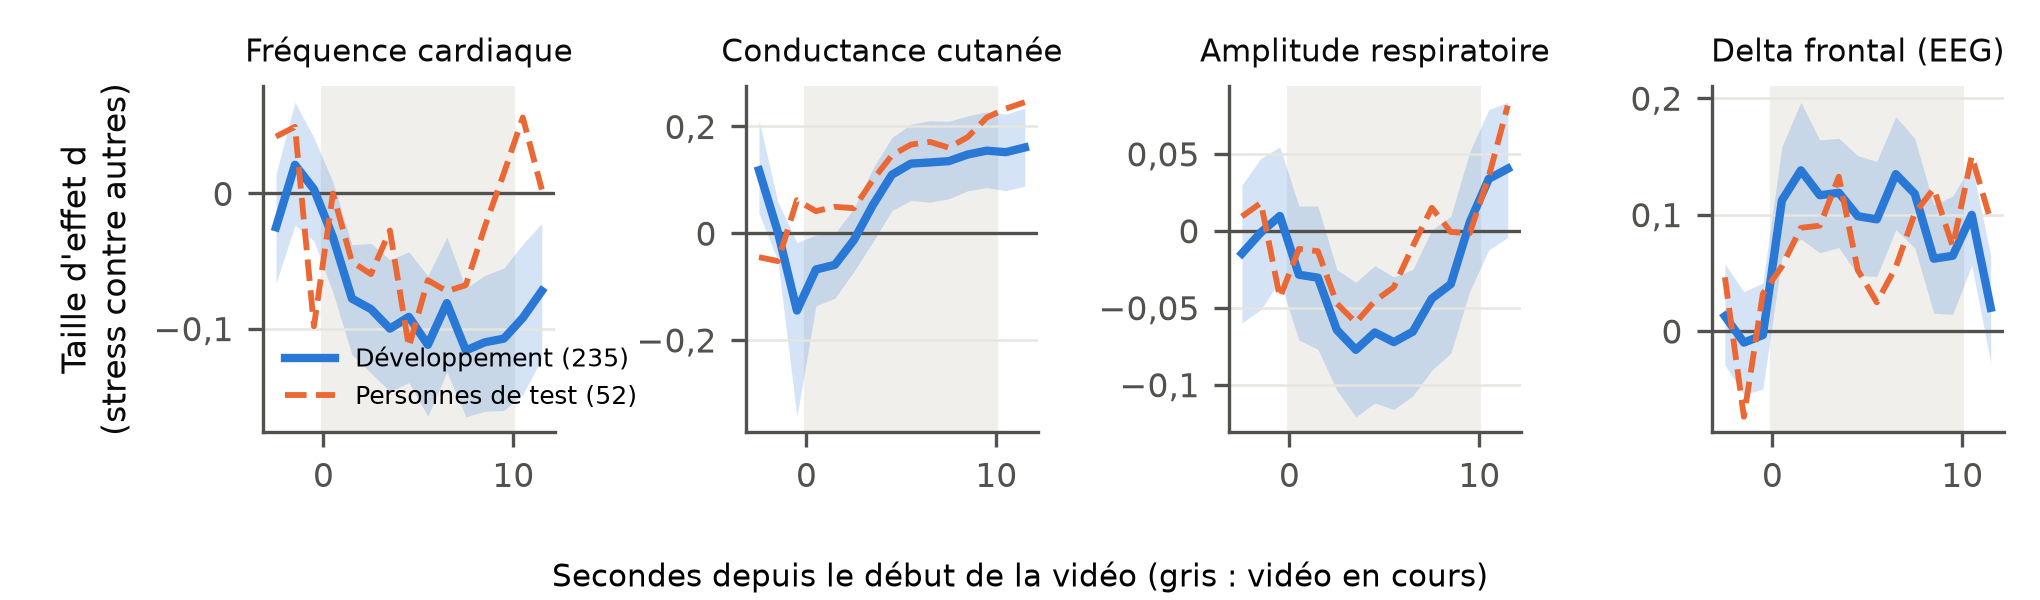
\includegraphics[width=0.92\linewidth]{curves_fr.png}
\caption{\textbf{Cascade temporelle seconde par seconde du stress aigu (Étude 05).} Taille d'effet intra-personne (stress vs autres essais, rapportée aux 3~s pré-stimulus) : delta EEG $<1$~s, freinage cardiaque dès 1~s, respiration moins ample 2--6~s, conductance cutanée à partir de 4~s. Bleu : 235 sujets \texttt{dev} (IC 95\,\%) ; orange : réplication sur 52 sujets tenus à l'écart.}
\label{fig:curves}
\end{figure}

En résolution 1~s (figure~\ref{fig:curves}), les effecteurs s'enchaînent dans un ordre reproductible cohérent avec le décalage central--autonome décrit dans la littérature \cite{jomaa2026,bradley2009,benedek2010} : delta EEG dès 0--1~s ($+0{,}11$ à $+0{,}14$), décélération cardiaque dès 1~s (creux $-0{,}12$ à 7~s), respiration superficielle à 2--6~s, puis conductance cutanée à 4--10~s (répliquée à $+0{,}25$ sur 52 sujets externes). Comme montré par Schippers et al.\ \cite{schippers2018} et Munoz et al.\ \cite{munoz2015}, la fréquence cardiaque sur 10~s concorde fortement avec une fenêtre de 60~s ($r = 0{,}94$), alors que la RMSSD ultra-courte est peu fiable ($r = 0{,}43$ intra-session et $0{,}22$ entre phases de 5~s).

\begin{figure}[t]
\centering
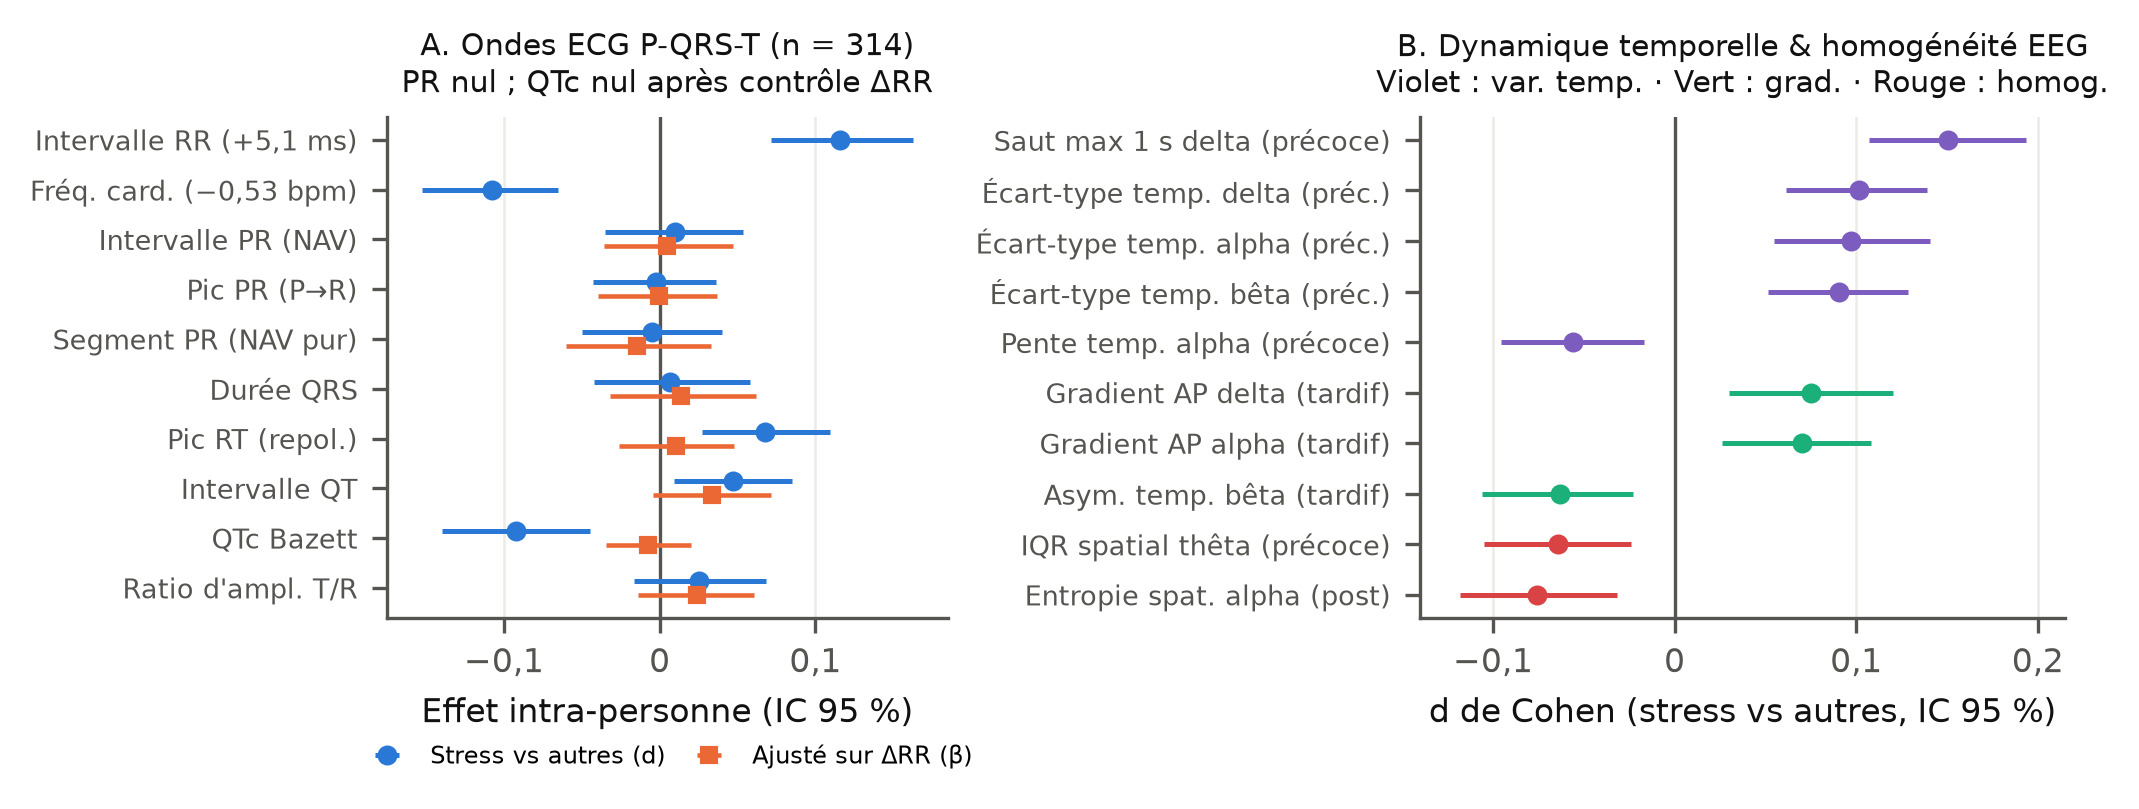
\includegraphics[width=0.98\linewidth]{fig3_ecg_eeg_rich_fr.png}
\caption{\textbf{Morphologie ECG P-QRS-T et descripteurs EEG enrichis (Étude 07).} \textbf{A.} Allongement net de l'intervalle RR ($+5{,}06$~ms) sans aucune variation du segment PR ($-0{,}04$~ms) ; la baisse apparente du QTc de Bazett disparaît après ajustement sur $\Delta\mathrm{RR}$. \textbf{B.} Hausse de la volatilité temporelle EEG précoce (saut delta $+0{,}151$) et réorganisation spatiale biphasique.}
\label{fig:ecg_eeg}
\end{figure}

La délinéation battement par battement (couverture 94,7--98,7\,\%, fiabilité 5~s $r = 0{,}45$--$0{,}71$, figure~\ref{fig:ecg_eeg}A) confirme directement le mécanisme vagal sino-atrial modélisé par Somsen et al.\ \cite{somsen2002} : l'intervalle RR s'allonge de $+5{,}06$~ms ($d = +0{,}116$ [$+0{,}071 ; +0{,}163$]), tandis que le pic PR ($-0{,}05$~ms, $d = -0{,}002$), le PR clinique ($+0{,}06$~ms), le segment PR pur ($-0{,}04$~ms, excluant toute accélération adrénergique marquée au nœud atrio-ventriculaire), QRS ($+0{,}007$) et le ratio T/R ($+0{,}025$) restent strictement nuls. La baisse apparente du QTc de Bazett ($d = -0{,}092$, $-1{,}00$~ms) est un artefact pur de formule qui s'annule après contrôle sur $\Delta\mathrm{RR}$ ($-0{,}007$ [$-0{,}035 ; +0{,}020$]). En parallèle, le potentiel évoqué cardiaque (HEP, 250--600~ms, $N = 287$, $\approx 13$ battements/essai) est identiquement nul sur l'EEG nettoyé par ICA ($d = +0{,}039$) et sur l'EEG brut \texttt{CURATED} sans ICA ($d = +0{,}038$ ; différence exacte retirée par l'ICA $+0{,}012$, $r = -0{,}004$ avec l'ECG), écartant l'hypothèse d'un signal cerveau--cœur effacé par l'ICA \cite{parkblanke2019}. En EEG, la volatilité temporelle précoce grimpe dans les cinq bandes (saut 1~s en delta $d = +0{,}151$ [$+0{,}107 ; +0{,}193$]), accompagnée d'une homogénéisation spatiale précoce suivie d'une focalisation post-clip (entropie spatiale alpha $-0{,}076$, figure~\ref{fig:ecg_eeg}B).

\subsection{Évaluation individuelle à vidéo fixe, sensibilité EEG et dynamique intra-clip par émotion}

\begin{figure}[t]
\centering
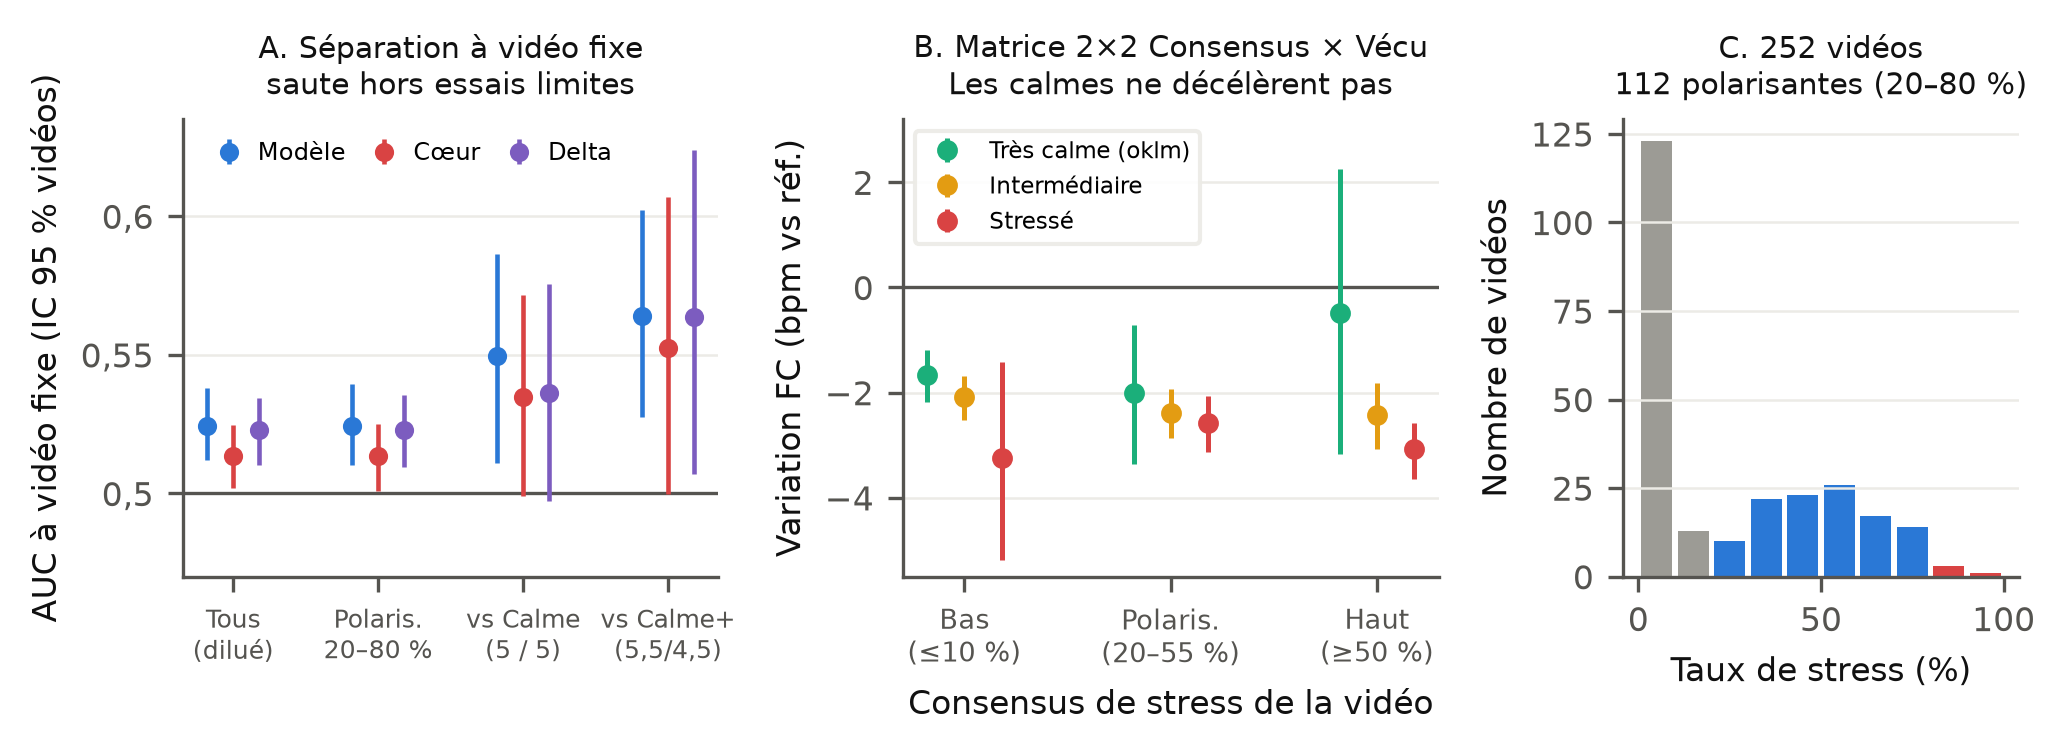
\includegraphics[width=0.98\linewidth]{fig5_fixed_video_fr.png}
\caption{\textbf{Contraste à vidéo fixe non adjacent et matrice $2\times 2$ Consensus $\times$ État vécu (Étude 07).} \textbf{A.} Retirer les spectateurs proches du seuil porte l'AUC à vidéo fixe de 0,525 à 0,564. \textbf{B.} Les spectateurs très calmes devant une vidéo stressante ne ralentissent pas leur cœur ($-0{,}49$~bpm vs $-3{,}08$~bpm chez les stressés). \textbf{C.} Répartition des taux de stress sur les 252 clips.}
\label{fig:fixed_video}
\end{figure}

Sur les vidéos consensuellement stressantes ($p_{v,-i} \ge 50\,\%$), 33,6\,\% des spectateurs « non stressés » sont en réalité proches du seuil et seuls 2,5\,\% restent vraiment calmes. En opposant stressés et spectateurs très calmes ($V \ge 5{,}5, A \le 4{,}5$) devant \emph{exactement la même vidéo} (48 clips, 6\,403 paires, figure~\ref{fig:fixed_video}), l'AUC à vidéo fixe monte de $0{,}525$ à \textbf{0,564} [$0{,}528 ; 0{,}602$] (delta $0{,}564$, FC $0{,}553$, EDA doublée à $d = +0{,}197$). Dans la matrice $2 \times 2$, les spectateurs très calmes devant une vidéo stressante ne montrent ni bradycardie ($-0{,}49$~bpm [$-3{,}16 ; +2{,}25$]) ni réponse EDA ($+0{,}014\,\mu$S), alors que les sujets stressés devant une vidéo neutre ralentissent de $-3{,}24$~bpm et élèvent l'EDA à $+0{,}071\,\mu$S. En comparaison appariée chez les mêmes individus ($N = 26$), l'effet évaluatif pur vaut $-2{,}97$~bpm ($d = -0{,}41$) sur le cœur et $+0{,}45$ sur le delta. À l'inverse, chez des sujets restés calmes devant des clips stressants vs neutres ($N = 29$), \textbf{seule la désynchronisation alpha occipitale se déclenche automatiquement} ($d = -0{,}33$ à $-0{,}41$), confirmant son rôle de filtrage attentionnel et de vigilance au stimulus plutôt que de marqueur spécifique du stress vécu \cite{zumer2014,panitz2019,bacigalupo2022,codispoti2023,stegmann2024,simons2009,kim2021,romeo2022}. La sensibilité évaluative propre (part propre résidualisée sur la vidéo) culmine en gamma frontal ($\beta_{\text{propre}} = -0{,}039$), bêta frontal ($-0{,}035$) et delta centro-pariétal ($-0{,}037$, intact à 93\,\% après contrôle oculaire pré-ICA sur Fp1/Fp2), tandis que l'asymétrie alpha frontale (FAA) est nulle ($+0{,}021$ \cite{vandervinne2017}). Au niveau trait ($N = 314$), une sensibilité subjective plus élevée corrèle avec une FC basale plus haute ($r = +0{,}140$), un gamma basal élevé ($+0{,}165$ \cite{oathes2008}) et le sexe féminin ($+0{,}172$ \cite{bradley2001}).

L'analyse directe par émotion déclarée (Études~07 et~10F, $N = 209$, $n = 17\,142$, figure~\ref{fig:coh_wclip}C) démontre l'hétérogénéité interne des émotions négatives \cite{qin2023,siegel2018,collet1997} et teste directement la dynamique intra-clip précoce $[0 ; 5)$~s vs tardive $[5 ; 10)$~s de Si et al.\ \cite{si2026} :
\begin{itemize}
\item \textbf{Peur ($n = 1\,425$ vs neutre) :} suppression alpha occipitale soutenue ($E = -0{,}118$, $L = -0{,}121$), respiration superficielle précoce ($E = -0{,}135$), bradycardie qui s'approfondit ($E = -0{,}144 \to L = -0{,}227$), et explosion électrodermale tardive ($E = +0{,}049$ NS $\to L = +0{,}289$ [$+0{,}174 ; +0{,}404$], transition $L - E = +0{,}341$).
\item \textbf{Dégoût ($n = 1\,816$ vs neutre) :} pic delta précoce massif ($E = +0{,}222$ [$+0{,}135 ; +0{,}311$] $\to L = +0{,}098$, aligné avec Si et al.\ \cite{si2026} et Alasfour \& AlSabah \cite{alasfour2025}), bradycardie vagale précoce ($-0{,}194$), EDA plate ($+0{,}070$ NS), mais — nuance importante face à Si et al.\ \cite{si2026} — une hausse tardive du gamma global ($+0{,}160$) et frontal ($+0{,}111$). En contraste direct \textbf{Peur $-$ Dégoût} ($N = 159$), le dégoût domine le delta centro-pariétal précoce ($-0{,}098$ [$-0{,}185 ; -0{,}001$]) et la transition gamma/bêta frontale tardive ($-0{,}178$ [$-0{,}273 ; -0{,}079$], possiblement nourrie par une micro-activité faciale/musculaire de grimace résiduelle), alors que la peur domine massivement l'EDA tardive ($+0{,}193$, transition $+0{,}303$ [$+0{,}197 ; +0{,}409$]), la suppression alpha tardive ($-0{,}137$) et l'accentuation bradycardique ($L - E = -0{,}104$).
\item \textbf{Autres états et clustering non supervisé :} la colère ($n = 1\,453$) élève le delta précoce ($+0{,}121$) et l'EDA tardive ($+0{,}103$) ; la tristesse ($n = 1\,470$) élève l'alpha occipital ($+0{,}104 / +0{,}132$) et laisse l'EDA plate ; la joie accélère le cœur en tardif ($+0{,}093$) ; la relaxation approfondit la respiration ($+0{,}205 / +0{,}186$) et synchronise l'alpha ($+0{,}119$). Enfin, le clustering non supervisé ($k$-means, GMM) échoue totalement à retrouver le stress ou les émotions ($\mathrm{ARI} < 0{,}009$, $\mathrm{NMI} \le 0{,}0015$, dix fois plus lié à la vidéo qu'au ressenti).
\end{itemize}

\begin{table}[t]
\centering\footnotesize
\begin{tabularx}{\linewidth}{@{}L{2.8cm} Y L{4.6cm}@{}}
\toprule
Axe physiologique & Résultat vérifié sur 314 personnes (22\,974 essais) & Chiffres clés (IC 95\,\%)\\
\midrule
Critère V/A et seuil & 89,2\,\% nég.\ rang~1 (97,2\,\% rangs 1--3) ; durcir double EDA/$\delta$ mais réduit la bradycardie. & Opt.\ $3/7$ (AUC $0{,}549$) ; EDA $+0{,}14 \to +0{,}34$, FC $-0{,}11 \to -0{,}04$.\\
ECG P-QRS-T \& HEP & Freinage vagal sinusal pur ; PR nul ; QTc artefact de Bazett ; HEP nul avec/sans ICA. & RR $+5{,}06$~ms ; PR $-0{,}05$~ms ; QTc adj.\ $-0{,}007$ ; HEP $+0{,}038$ vs $+0{,}039$.\\
Vidéo fixe \& $2\times 2$ & Retirer les cas limites révèle l'évaluation ; seule l'alpha occipitale est automatique. & AUC SV $0{,}525 \to 0{,}564$ ; apparié FC $-2{,}97$~bpm ($d=-0{,}41$) ; $\alpha$ calme $-0{,}41$.\\
Dynamique intra-clip & Dégoût = $\delta$ précoce + $\gamma$ tardif ; Peur = $\alpha$ soutenu + FC + explosion EDA tardive. & Peur$-$Dégoût : $\delta_{\text{CP}}$ $-0{,}098^*$, EDA $L-E$ $+0{,}303^*$, $\alpha$ $-0{,}137^*$, $\gamma_{\text{fr}}$ $-0{,}178^*$.\\
\bottomrule
\end{tabularx}
\caption{Synthèse de l'architecture neurophysiologique du stress aigu bref (Études 05--07 et 10F).}
\label{tab:physio}
\end{table}

\section{Information prédictive causale de l'EEG précoce sur la physiologie future (Étude 09)}
\label{sec:forecast}

\subsection{Quantification des fuites antérieures et dissociation organe M2 contre M0}

L'audit quantitatif des Études~07--08 confirme deux sources majeures de surestimation (tableau~\ref{tab:forecast_audit}) : le centrage transductif global gonflait la régression logistique de stress de $+0{,}0141$ ($0{,}5564 \to 0{,}5705$), et le passage bidirectionnel de \texttt{REVE-base} sur 13~s couplé aux 77\,\% de thèmes vus gonflait \texttt{M1} ($\text{EEG} \to \text{Corps}[5 ; 10)$~s) de $+0{,}0588$ sur l'ECG ($0{,}2638 \to 0{,}2050$), $+0{,}0424$ sur l'EDA et $+0{,}0689$ sur la respiration.

\begin{figure}[t]
\centering
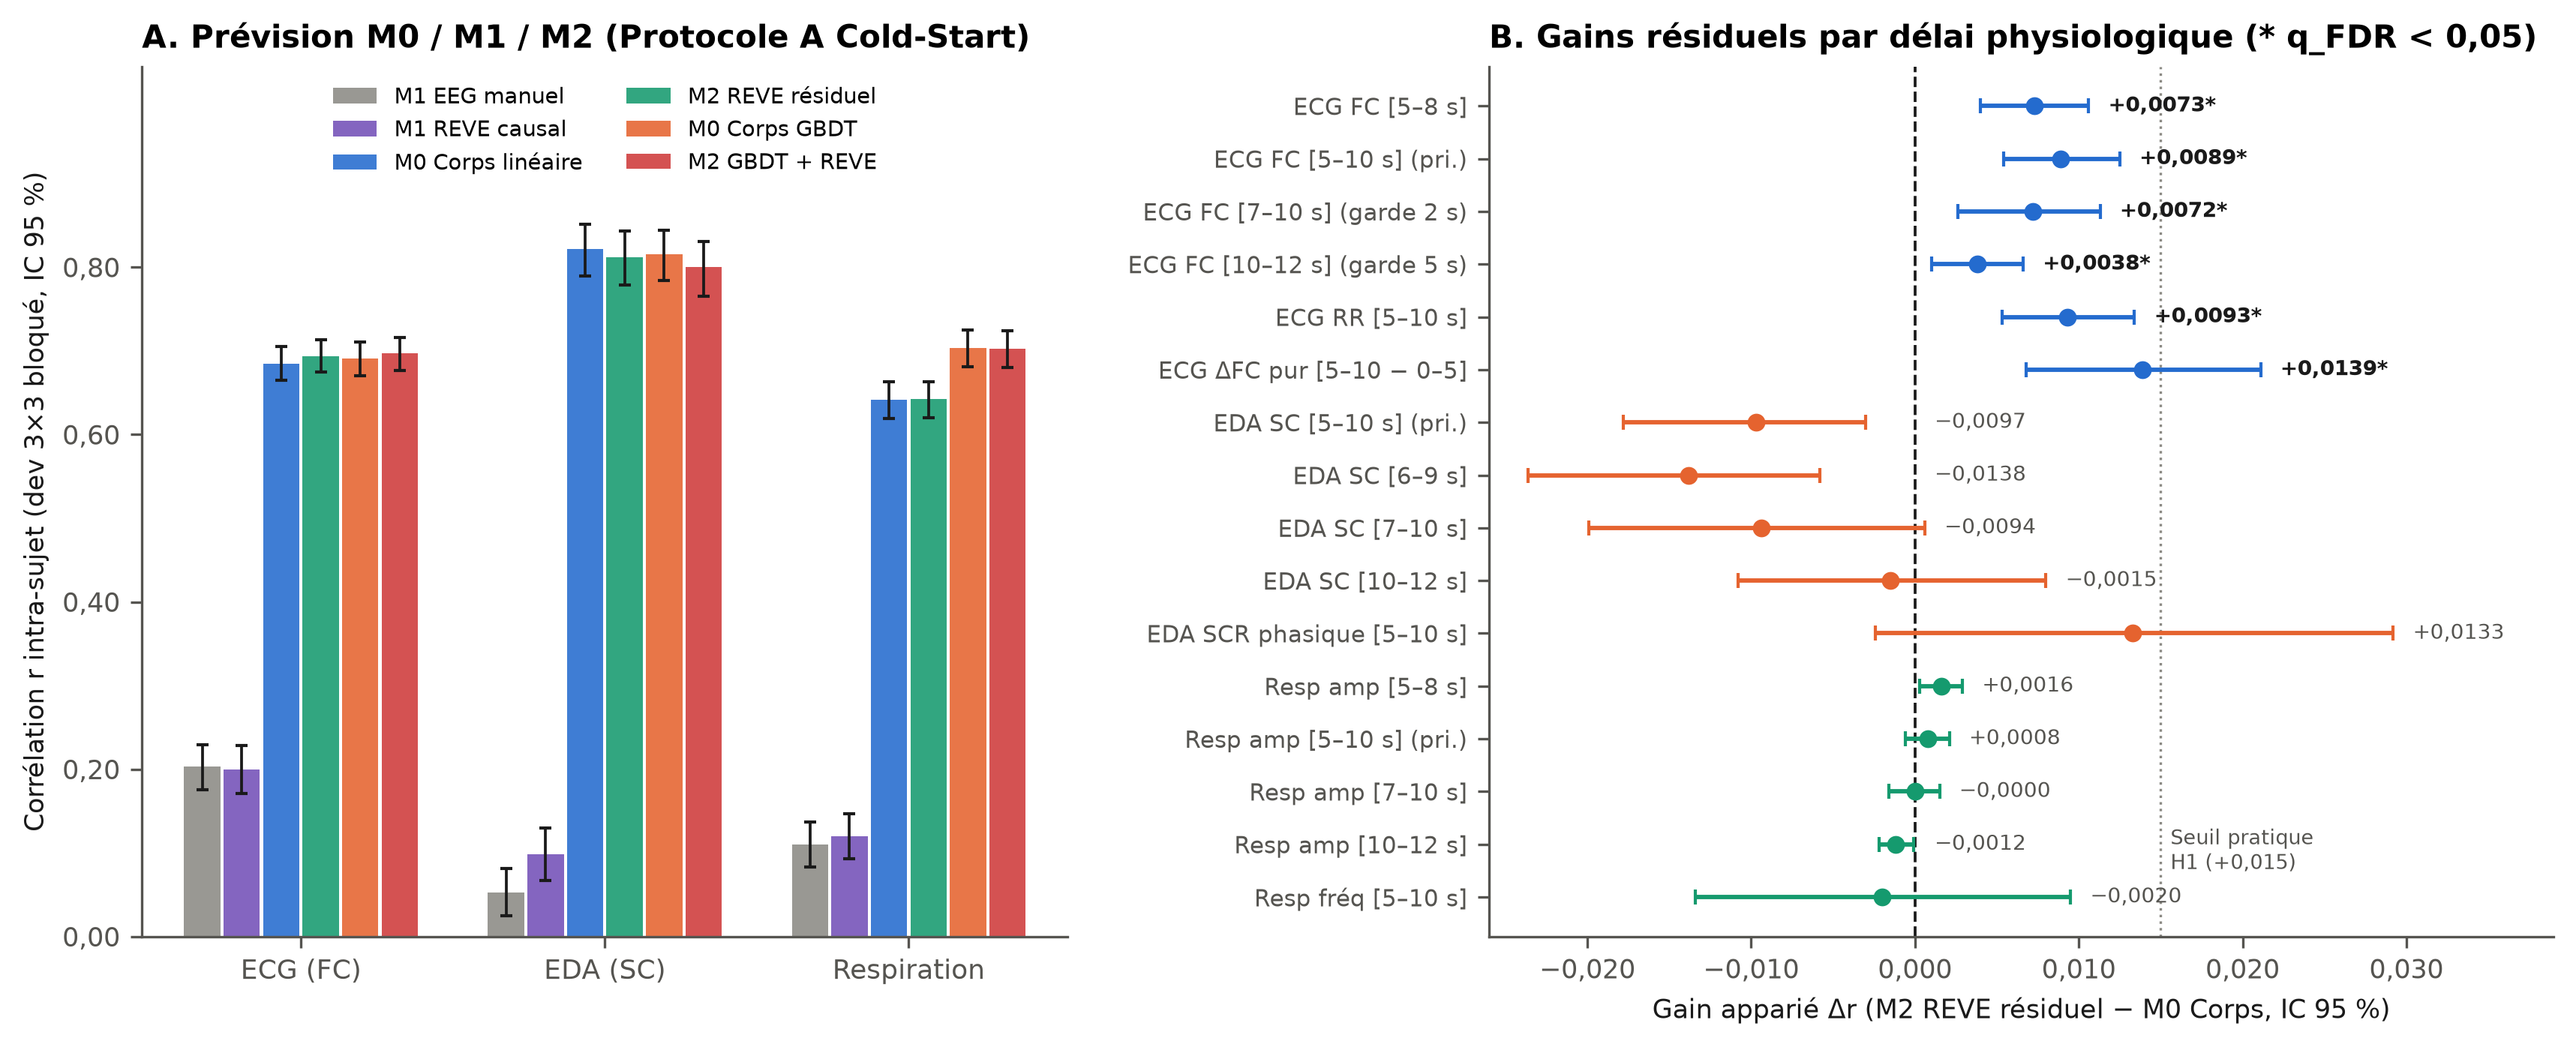
\includegraphics[width=0.98\linewidth]{fig2_forecast_delays_fr.png}
\caption{\textbf{Prévision causale \texttt{M0 / M1 / M2} sous mur causal dur à $t = 5{,}000$~s (\texttt{dev} $3\times 3$, Cold-Start, Étude 09).} \textbf{A.} Corrélation $r$ intra-sujet par organe et famille (incluant le contrôle non linéaire GBDT). \textbf{B.} Gains appariés $\Delta r$ (\texttt{M2\_reve\_resid $-$ M0\_linear}, IC 95\,\%) sur les 16 cibles et délais physiologiques (* : $q_{\text{FDR}} < 0{,}05$ et borne inf.\ $> 0$).}
\label{fig:forecast}
\end{figure}

Sous mur causal strict à $t = 5{,}000$~s en Cold-Start (\texttt{dev} $3\times 3$), comparer \texttt{M2} ($(\text{EEG}+\text{Corps})[0 ; 5)$) à \texttt{M0} ($\text{Corps}[0 ; 5)$ seul) tranche nettement la question par organe (figure~\ref{fig:forecast} et tableau~\ref{tab:forecast_audit}) :
\begin{itemize}
\item \textbf{Dynamique cardiaque (ECG, $N = 224$) : gain prédictif réel, cohérent mais modeste.} Au-delà de \texttt{M0\_linear} ($r = 0{,}6849$), l'EEG précoce améliore significativement toutes les architectures : EEG manuel résiduel $+0{,}0071$, \texttt{M2\_reve\_resid} \textbf{$+0{,}0089$} [$+0{,}0054 ; +0{,}0125$] (67,0\,\% améliorés, $q_{\text{FDR}} < 10^{-6}$), \texttt{M2\_reve\_joint} \textbf{$+0{,}0110$} [$+0{,}0065 ; +0{,}0156$] (\textbf{71,4\,\%} améliorés, $\Delta R^2_{\text{intra}} = +0{,}0149$), sensibilité $5 \times 5$ \textbf{$+0{,}0120$}, et contrôle non linéaire \texttt{M2\_gbdt $-$ M0\_gbdt} \textbf{$+0{,}0063$} [$+0{,}0021 ; +0{,}0102$] ($p = 7{,}3 \times 10^{-4}$). Le gain est maximal sur l'incrément cardiaque pur $\Delta\mathrm{FC}_{[5;10)-[0;5)}$ (\textbf{$+0{,}0182$} [$+0{,}0086 ; +0{,}0276$]), confirmé sur RR ($+0{,}0093$, 72\,\%), et persiste après bande de garde de 2~s ($[7 ; 10)$~s : $+0{,}0089$) et 5~s ($[10 ; 12)$~s : $+0{,}0038$ [$+0{,}0010 ; +0{,}0066$]). Il demeure néanmoins inférieur au seuil pratique pré-enregistré de $+0{,}015$ sur la cible primaire : $\approx 97$--$98\,\%$ de la variance prévisible provient déjà du passé périphérique.
\item \textbf{Conductance cutanée ($N = 200$) et respiration ($N = 228$) : réfutation complète.} Sur l'EDA (\texttt{M0\_linear} $r = 0{,}8218$), ajouter l'EEG dégrade la prévision ($-0{,}0097$ résiduel, $-0{,}0155$ en GBDT) sur toutes les fenêtres. Sur la respiration, l'EEG linéaire est nul ($+0{,}0008$, $q = 0{,}346$), et le contrôle non linéaire \texttt{M0\_gbdt} seul bondit de $0{,}6417$ à \textbf{0,7036} sans aucun ajout de l'EEG (\texttt{M2\_gbdt $-$ M0\_gbdt} $= -0{,}0008$, $p = 0{,}453$), démasquant un faux positif apparent ($+0{,}0096$) d'une tête neuronale comparée au seul modèle linéaire.
\end{itemize}

\begin{table}[t]
\centering\scriptsize\setlength{\tabcolsep}{3.5pt}
\begin{tabular}{@{}llrrrr@{}}
\toprule
Cible / Audit & Modèle ou Régime & $r$ / AUC & $\Delta$ vs réf.\ [IC 95\,\%] & \% amél. & $p$ / $q_{\text{FDR}}$\\
\midrule
Audit fuites & S07 LogReg Cold-Start $\to$ Global & $0{,}556 \to 0{,}571$ & $+0{,}0141$ (fuite) & — & —\\
(Études 07--08) & \texttt{M1 REVE} bidir.\ 13~s $\to$ causal & $0{,}264 \to 0{,}205$ & $-0{,}059$ / $-0{,}042$ / $-0{,}069$ & — & —\\
\midrule
ECG FC $[5;10)$~s & \texttt{M0\_lin} $\to$ \texttt{M2\_resid} / \texttt{joint} & $0{,}685 \to \mathbf{0{,}696}$ & $\mathbf{+0{,}0089}$ / $\mathbf{+0{,}0110}$ [$+0{,}007 ; +0{,}016$] & \textbf{71,4\,\%} & $<10^{-6}$\\
($N = 224$) & \texttt{M0\_gbdt} $\to$ \texttt{M2\_gbdt\_reve} & $0{,}691 \to \mathbf{0{,}697}$ & $\mathbf{+0{,}0063}$ [$+0{,}002 ; +0{,}010$] & 57,6\,\% & $7{,}3\times 10^{-4}$\\
 & Incrément pur $\Delta\mathrm{FC}$ (\texttt{joint}) & $0{,}210 \to 0{,}228$ & $\mathbf{+0{,}0182}$ [$+0{,}009 ; +0{,}028$] & 63,4\,\% & $<10^{-5}$\\
 & \textbf{LOCO 5/5 cohortes} (\texttt{M2\_resid}) & $0{,}689 \to \mathbf{0{,}699}$ & $\mathbf{+0{,}0107}$ [$+0{,}007 ; +0{,}015$] & \textbf{68,8\,\%} & $<10^{-6}$\\
\midrule
EDA SC ($N=200$) & \texttt{M0\_lin} / \texttt{M2\_resid} / \texttt{M2\_gbdt} & $\mathbf{0{,}822}$ / $0{,}812$ / $0{,}800$ & $-0{,}0097$ / $-0{,}0155$ & 45,0\,\% & réfutée\\
Resp ($N=228$) & \texttt{M0\_lin} / \texttt{M0\_gbdt} $\to$ \texttt{M2\_gbdt} & $0{,}642$ / $\mathbf{0{,}704} \to 0{,}703$ & $+0{,}0008$ / $-0{,}0008$ & 46,9\,\% & réfutée\\
\bottomrule
\end{tabular}
\caption{Audit des fuites et bilan de la prévision causale \texttt{M0 / M1 / M2} (Études 09 et 10C).}
\label{tab:forecast_audit}
\end{table}

\subsection{Contrôles d'artefacts, temporels, négatifs et preuve d'idiosyncrasie}

\begin{figure}[t]
\centering
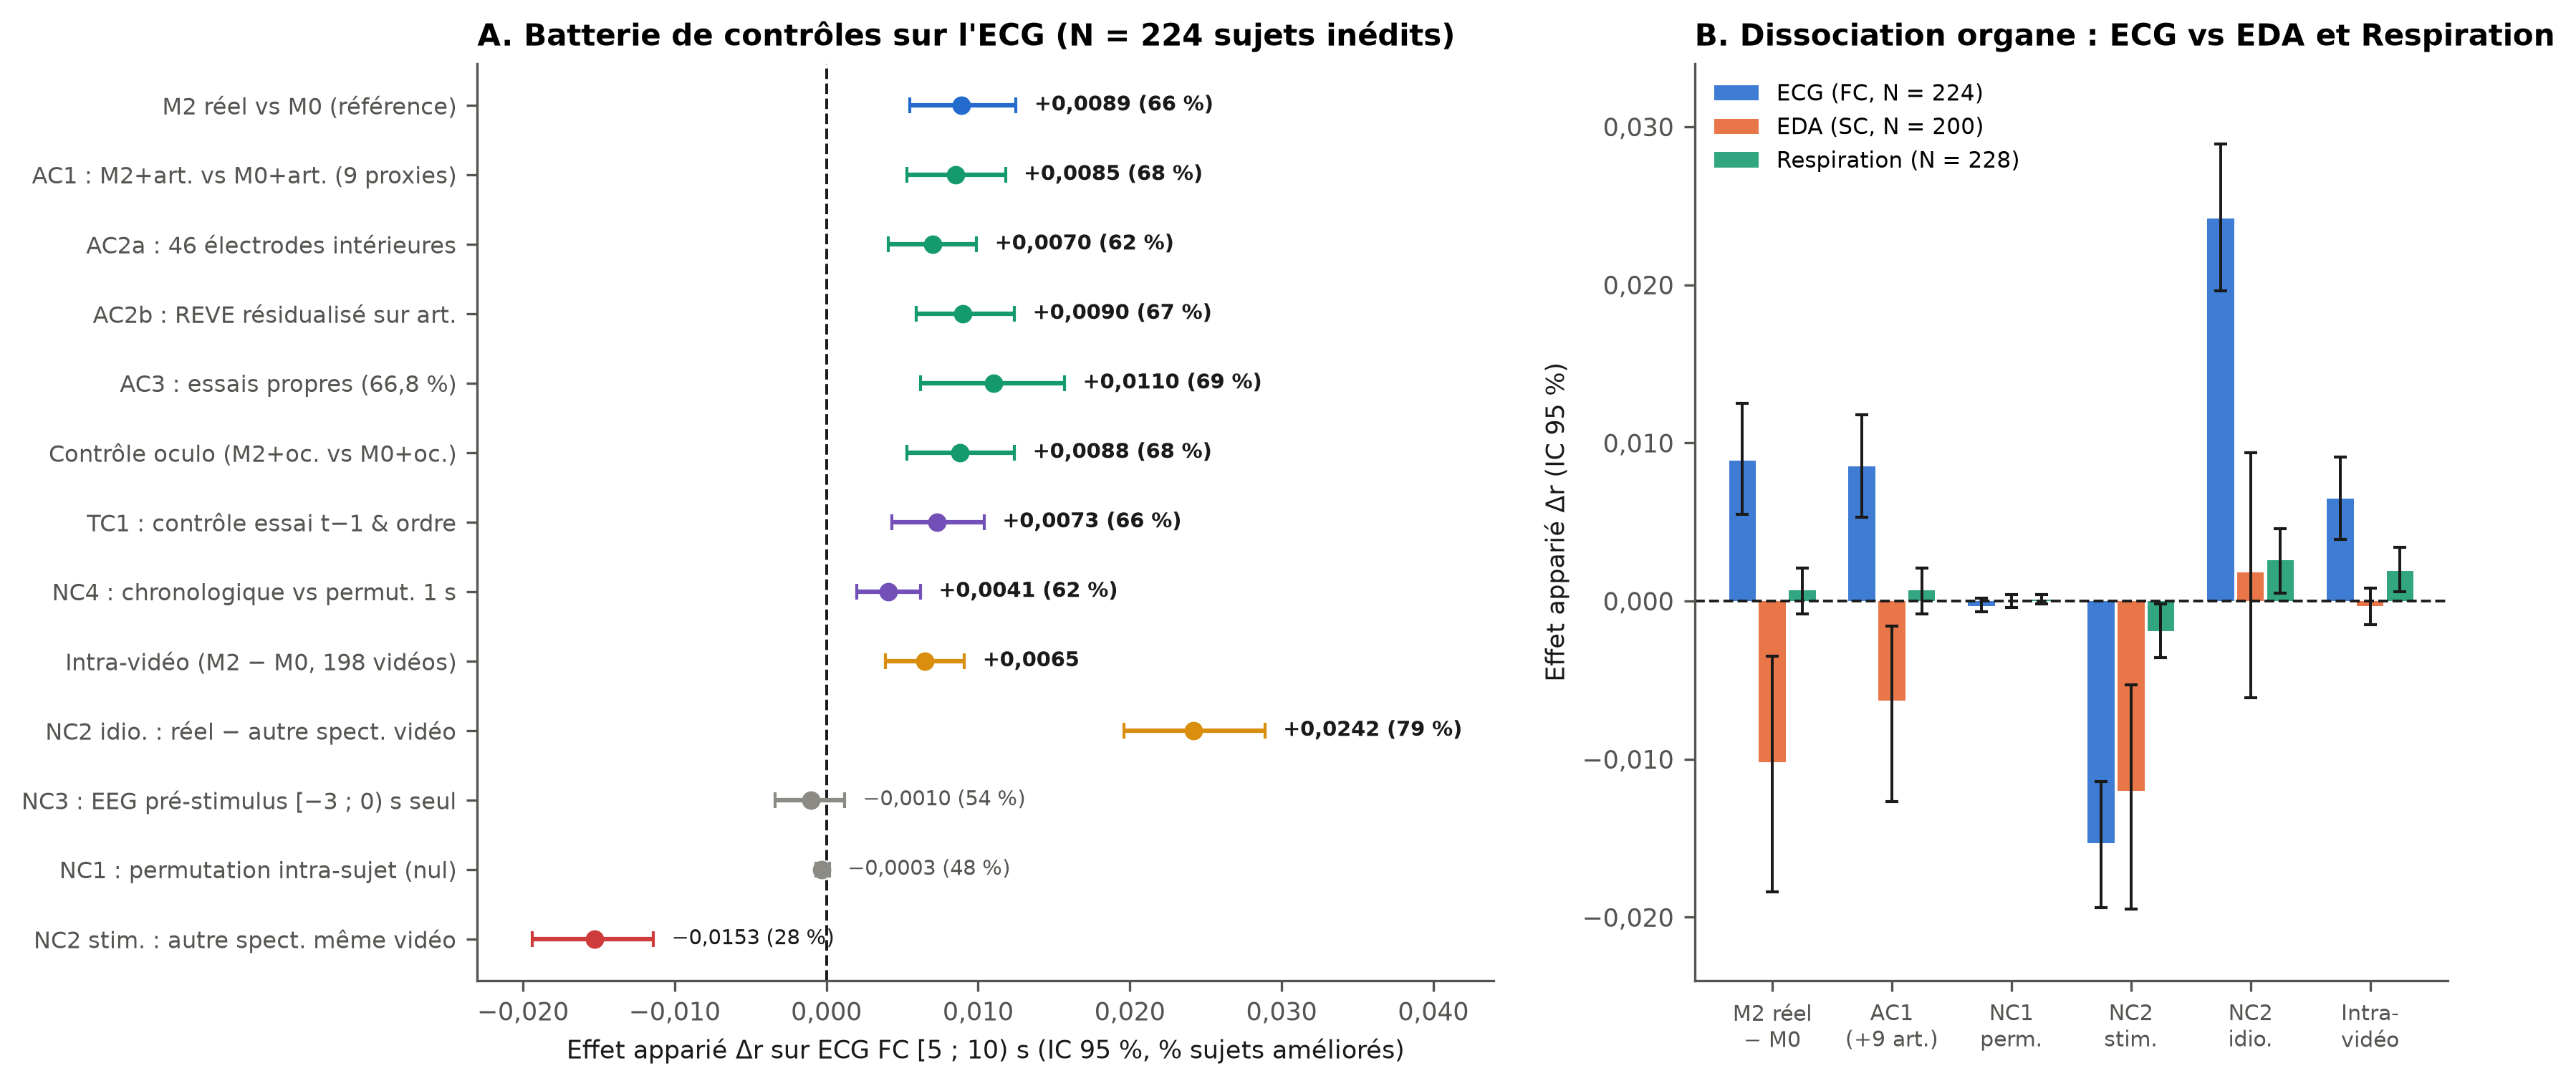
\includegraphics[width=0.98\linewidth]{fig3_controls_fr.png}
\caption{\textbf{Batterie des 12 contrôles sur la prévision causale (Étude 09).} \textbf{A.} Sur l'ECG ($N = 224$), le gain résiste aux 9 covariables d'artefacts (\texttt{AC1}), aux 46 électrodes intérieures (\texttt{AC2a}), augmente sur essais propres (\texttt{AC3}), résiste à l'essai $t-1$ (\texttt{TC1}), s'annule en permutation intra-sujet (\texttt{NC1}) et pré-stimulus (\texttt{NC3}), dépend de l'ordre temporel (\texttt{NC4}) et s'inverse si l'on substitue l'EEG d'un autre spectateur de la même vidéo (\texttt{NC2}). \textbf{B.} Spécificité cardiaque face à l'EDA et à la respiration.}
\label{fig:controls}
\end{figure}

Les douze contrôles pré-enregistrés (figure~\ref{fig:controls}) établissent que le signal cardiaque n'est ni un artefact ni un raccourci de reconnaissance vidéo : le détecteur de fuite \textbf{NC1} vaut exactement zéro ($-0{,}0003$), le pré-stimulus seul \textbf{NC3} est nul ($-0{,}0010$), le contrôle des 9 proxies d'artefacts (\textbf{AC1} $+0{,}0085$), des 46 électrodes intérieures hors bordure (\textbf{AC2a} $+0{,}0070$), des 6 covariables oculométriques ($+0{,}0088$) et de l'essai précédent (\textbf{TC1} $+0{,}0073$) laissent le signal intact, les essais propres le renforcent (\textbf{AC3} $+0{,}0110$), et la permutation chronologique 1~s l'efface (\textbf{NC4} $+0{,}0041$). Surtout, \textbf{NC2} tranche l'origine individuelle : substituer l'EEG par celui d'un autre spectateur regardant \emph{exactement la même vidéo} fait chuter le score sous \texttt{M0} ($-0{,}0153$), portant le contraste idiosyncrasique réel $-$ autre spectateur à \textbf{$+0{,}0242$} (79,0\,\% améliorés) et le gain strictement intra-vidéo à \textbf{$+0{,}0065$} [$+0{,}0039 ; +0{,}0091$] sur 198 clips. Comme démontré en Étude~10C (figure~\ref{fig:longit}C), ce couplage central--vagal prédictif \cite{thayer2009} se réplique positivement dans \textbf{les 5 cohortes HABS évaluées hors-cohorte (LOCO-CV)} : $+0{,}0048^*$ (C1), $+0{,}0150^*$ (C2), $+0{,}0069$ (C3), $+0{,}0157^*$ (C4) et $+0{,}0111$ (C5), soit \textbf{$+0{,}0107$} [$+0{,}0071 ; +0{,}0145$] globalement (68,8\,\% améliorés).

\section{Généralisation, modèles fondation, stabilité longitudinale et personnalisation (Études 08--10C)}
\label{sec:gen}

\subsection{Modèles fondation EEG, PhysioJEPA, LoRA, Trait/État et oculométrie}

Sur le décodage du stress subjectif (tableau~\ref{tab:ssl_ts}), nos Études~08 et~09 révèlent une double dissociation nette entre dynamique physiologique et étiquette subjective. D'un côté, l'apprentissage auto-supervisé améliore les dynamiques objectives : notre modèle du monde multimodal \texttt{PhysioJEPA} (0,90~M paramètres, 53~h \texttt{dev} sans étiquettes) surpasse son contrôle supervisé à capacité identique sur la prédiction continue d'affect ($\bar{\rho} : 0{,}055 \to 0{,}096$), la stabilité inter-seeds ($\pm 0{,}001$) et les sondes temporelles sans raccourci positionnel (flèche du temps $0{,}802$, effondrement au hasard $0{,}556 \to 0{,}484$ après permutation temporelle). De l'autre côté, face aux 4 phases linéaires enrichies de l'Étude~07 (0 GPU : $0{,}576$--$0{,}581$ en \texttt{dev} centré, $0{,}569$--$0{,}572$ en Cold-Start strict, $0{,}586$--$0{,}622$ sur tests scellés, $0{,}656$ contre relaxé), \textbf{aucun des cinq modèles fondation EEG (\texttt{REVE-base} 69,2~M \cite{reve2025}, \texttt{EEGPT}, \texttt{LaBraM}, \texttt{CBraMod}, \texttt{Signal-JEPA}), ni \texttt{PhysioJEPA}, ni l'adaptation LoRA \cite{hu2022} ($-0{,}0069$ vs tête gelée pour $21{,}7\times$ plus de temps GPU), ni le stacking OOF imbriqué ($-0{,}0084$)} n'apporte de gain de généralisation.

Trois enseignements techniques transférables émergent néanmoins de l'Étude~09 :
\begin{enumerate}
\item \textbf{Perte de ranking intra-sujet décisive :} retirer le terme de ranking par paires intra-sujet dans \texttt{REVE} multitâche fait chuter l'AUC Cold-Start de $0{,}5495$ à $0{,}5089$ (perte appariée $-0{,}0406$ [$-0{,}0544 ; -0{,}0266$]).
\item \textbf{Factorisation Trait/État par \emph{shrinkage} bayésien empirique :} les embeddings bruts de \texttt{REVE} encodent 51,0\,\% de variance biométrique d'identité (identification inter-jours J1$\to$J2 jusqu'à 45,4\,\% top-1 en multimodal \texttt{PhysioJEPA}). Soustraire aveuglément les 3~s pré-stimulus dégrade l'AUC ($0{,}5609 \to 0{,}5551$), tandis que le \emph{shrinkage} bayésien empirique réduit $R^2_{\text{sujet}}$ à 36,9\,\%, préserve intégralement l'AUC intra-sujet ($0{,}5605$), élève $\bar{\rho}$ ($0{,}0795 \to 0{,}0822$) et améliore la calibration (AUC poolée $0{,}5302 \to 0{,}5425$, Brier $0{,}2489 \to 0{,}2479$), sans que le sous-espace trait ANOVA ne prédise la sensibilité-trait subjective ($\rho = -0{,}113$).
\item \textbf{Audit oculométrique des 508 enregistrements :} 500/508 fichiers ont 96,5\,\% d'essais valides, une corrélation binoculaire médiane de $0{,}852$ et un saut instantané de vitesse du regard à $t = 0{,}00$~s ($+121$~px/s, $+19{,}4$~ET), prouvant l'alignement temporel ; mais le réflexe pupillaire moyen global échoue à la porte stricte ($-0{,}004$~mm, $p = 0{,}209$, luminance vidéo hétérogène) et les baselines oculaires simples restent au hasard en stress ($0{,}5058$).
\end{enumerate}

\begin{table}[t]
\centering\scriptsize\setlength{\tabcolsep}{4.5pt}
\begin{tabular}{@{}lrrrrrr@{}}
\toprule
Famille / Modèle (Études 08--09, \texttt{dev} $3\times 3$) & Protocole & AUC V\&A & AUC LogReg & $\bar{\rho}$ affect & $R^2_{\text{ID}}$ & Coût GPU\\
\midrule
\texttt{S07 enrichi} (4 phases linéaires, 448 var.) & Cold-Start & \textbf{0,5709} & 0,5564 & \textbf{0,0953} & 52,2\,\% & \textbf{0 s}\\
\texttt{REVE-base} gelé (sonde linéaire, 69,2~M) & Cold-Start & 0,5609 & \textbf{0,5641} & 0,0795 & 51,0\,\% & 43 s ext.\\
\texttt{REVE-base} + \emph{shrinkage} EB état seul & Cold-Start & 0,5605 & 0,5575 & 0,0822 & \textbf{36,9\,\%} & 0 s supp.\\
\texttt{REVE-base} tête gelée multitâche + ranking & Cold-Start & 0,5564 & 0,5543 & 0,0752 & — & 77 s\\
\texttt{REVE-base} LoRA $r=8$ multitâche + ranking & Cold-Start & 0,5495 & 0,5528 & 0,0625 & — & 1\,665 s\\
\texttt{REVE-base} LoRA $r=8$ \textbf{sans ranking} (\texttt{norank}) & Cold-Start & \textbf{0,5089} & 0,5166 & 0,0026 & — & 1\,665 s\\
\texttt{PhysioJEPA} (4 mod., 53~h SSL) vs \texttt{Scratch} & Centré É08 & 0,5623 / 0,5538 & — & 0,079 / 0,056 & 44,9\,\% & 1,03 H100-h\\
Oculométrie simple (10 var.\ causales) & Cold-Start & 0,5058 & 0,4801 & $-0{,}0007$ & — & 0 s\\
\bottomrule
\end{tabular}
\caption{Bilan comparé des modèles fondation EEG, du SSL, de LoRA + ranking, Trait/État et oculométrie (Études 08--09).}
\label{tab:ssl_ts}
\end{table}

\subsection{Échelle de généralisation R1--R4 et ablation de modalités (Étude 10A)}

\begin{figure}[t]
\centering
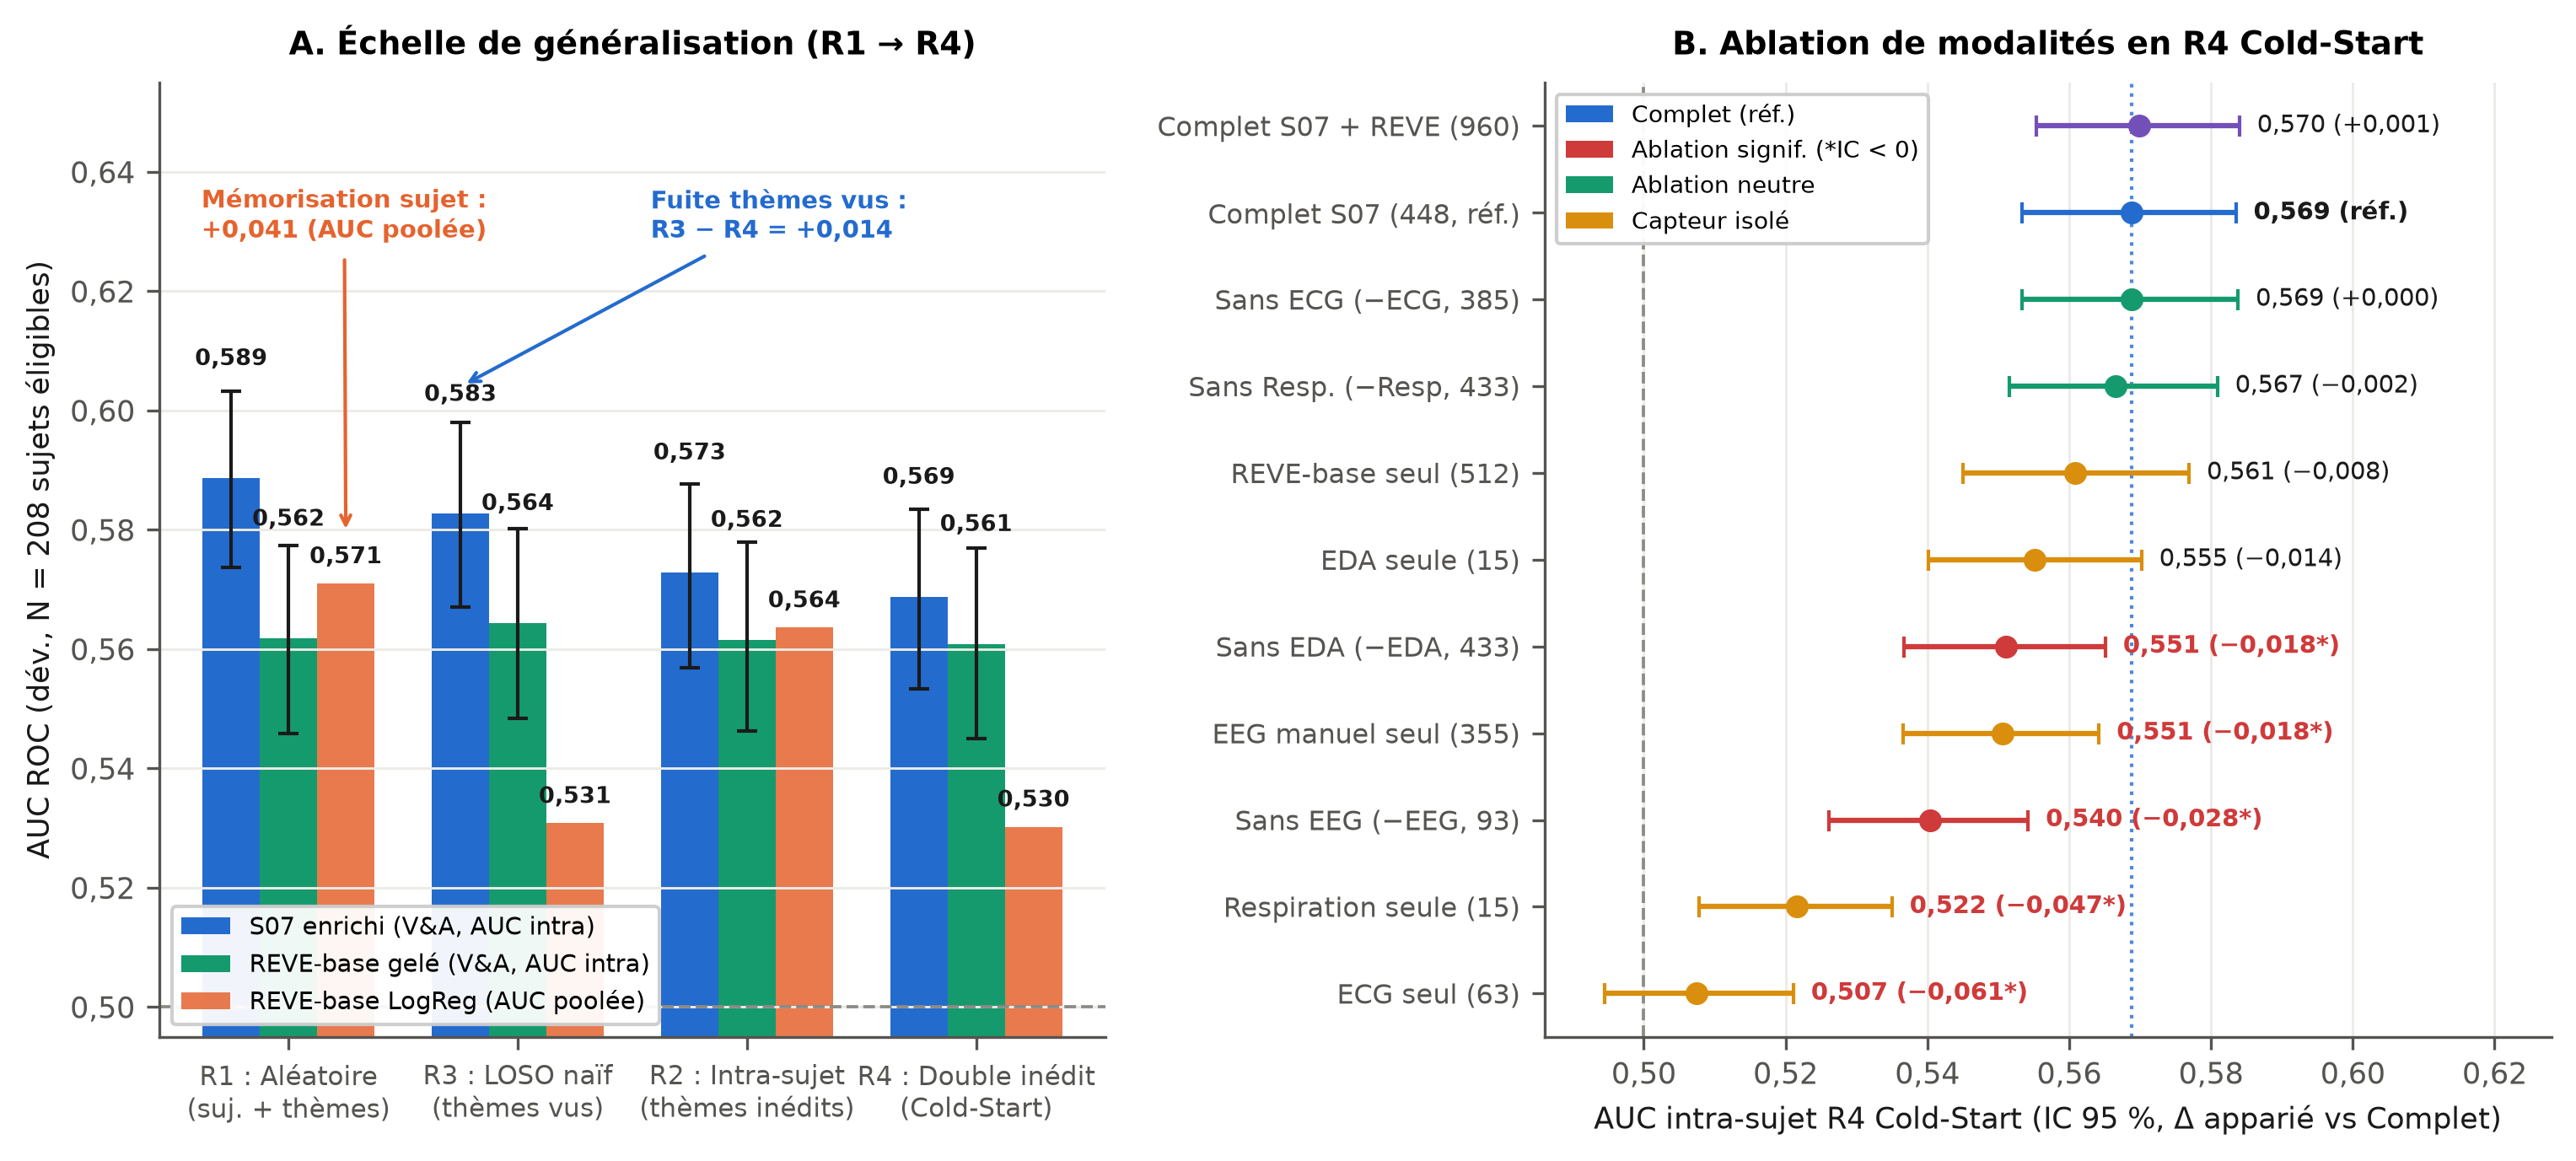
\includegraphics[width=0.98\linewidth]{fig1_generalization_ablation_fr.png}
\caption{\textbf{Échelle de généralisation R1 $\to$ R4 et ablation de modalités en R4 Cold-Start (Étude 10A, \texttt{dev}, $N = 208$).} \textbf{A.} Décomposition de l'optimisme entre split aléatoire (R1), LOSO naïf sur thèmes vus (R3), intra-sujet sur thèmes inédits (R2) et double inédit Cold-Start (R4). \textbf{B.} Contributions appariées des capteurs en R4 : seules les ablations de l'EEG ($-0{,}028^*$) et de l'EDA ($-0{,}018^*$) dégradent significativement le détecteur.}
\label{fig:gen_abl}
\end{figure}

Conformément aux diagnostics d'Alshamrani \cite{alshamrani2026}, Hinduja et al.\ \cite{hinduja2023} et Li et al.\ \cite{li2026}, la figure~\ref{fig:gen_abl}A dissèque l'écart entre validations permissives et double inédit strict (\textbf{R4}) sur le même jeu \texttt{dev} ($N = 208$). Pour \texttt{S07 enrichi} (Ridge V\&A), l'AUC intra-sujet glisse de \textbf{0,5887} (R1 aléatoire, vs relaxé 0,619, $\bar{\rho} = 0{,}124$) à \textbf{0,5827} (R3 LOSO sur thèmes vus), \textbf{0,5729} (R2 intra-sujet, thèmes inédits) et \textbf{0,5688} (R4 double inédit Cold-Start, vs relaxé 0,585, $\bar{\rho} = 0{,}097$) : \textbf{70\,\% du biais du split aléatoire provient du partage de thèmes vidéo} ($\text{R3} - \text{R4} = +0{,}0139$), un raccourci d'identité de stimulus concordant avec Gerster et al.\ \cite{gerster2026}. Pour \texttt{REVE-base} en régression logistique directe, le split aléatoire gonfle l'AUC poolée de \textbf{+0,0408} ($0{,}5302 \to 0{,}5710$) par mémorisation biométrique du sujet.

L'ablation stricte sur R4 Cold-Start (figure~\ref{fig:gen_abl}B) apporte un contraste éclairant avec Alshamrani \cite{alshamrani2026} (où la suppression cardiaque coûtait 42 points sur tâches motrices/physiques) : sur 10~s de visionnage passif, la courbe cardiaque en U rend l'ECG seul quasi nul en Cold-Start ($0{,}5075$ [$0{,}495 ; 0{,}521$]) et la respiration faible ($0{,}5216$). À l'inverse, \textbf{l'EEG et l'EDA constituent deux piliers significatifs et complémentaires} \cite{coelli2026} : retirer l'EEG fait chuter l'AUC de \textbf{$-0{,}0284$} [$-0{,}0429 ; -0{,}0144$] ($0{,}5688 \to 0{,}5404$), retirer l'EDA la fait chuter de \textbf{$-0{,}0177$} [$-0{,}0259 ; -0{,}0097$] ($0{,}5688 \to 0{,}5511$), tandis que retirer l'ECG ($0{,}0000$) ou la respiration ($-0{,}0023$) est neutre. Le multimodal complet (\texttt{All} $0{,}5688$, \texttt{All + REVE} $0{,}5699$, LogReg $0{,}5714$) bat chaque capteur pris séparément (\texttt{REVE} $0{,}5609$, \texttt{EDA} $0{,}5551$, \texttt{EEG manuel} $0{,}5506$).

\subsection{Stabilité longitudinale J1--J2, habituation, personnalisation k-shot et LOCO (Études 10B--C)}

\begin{figure}[t]
\centering
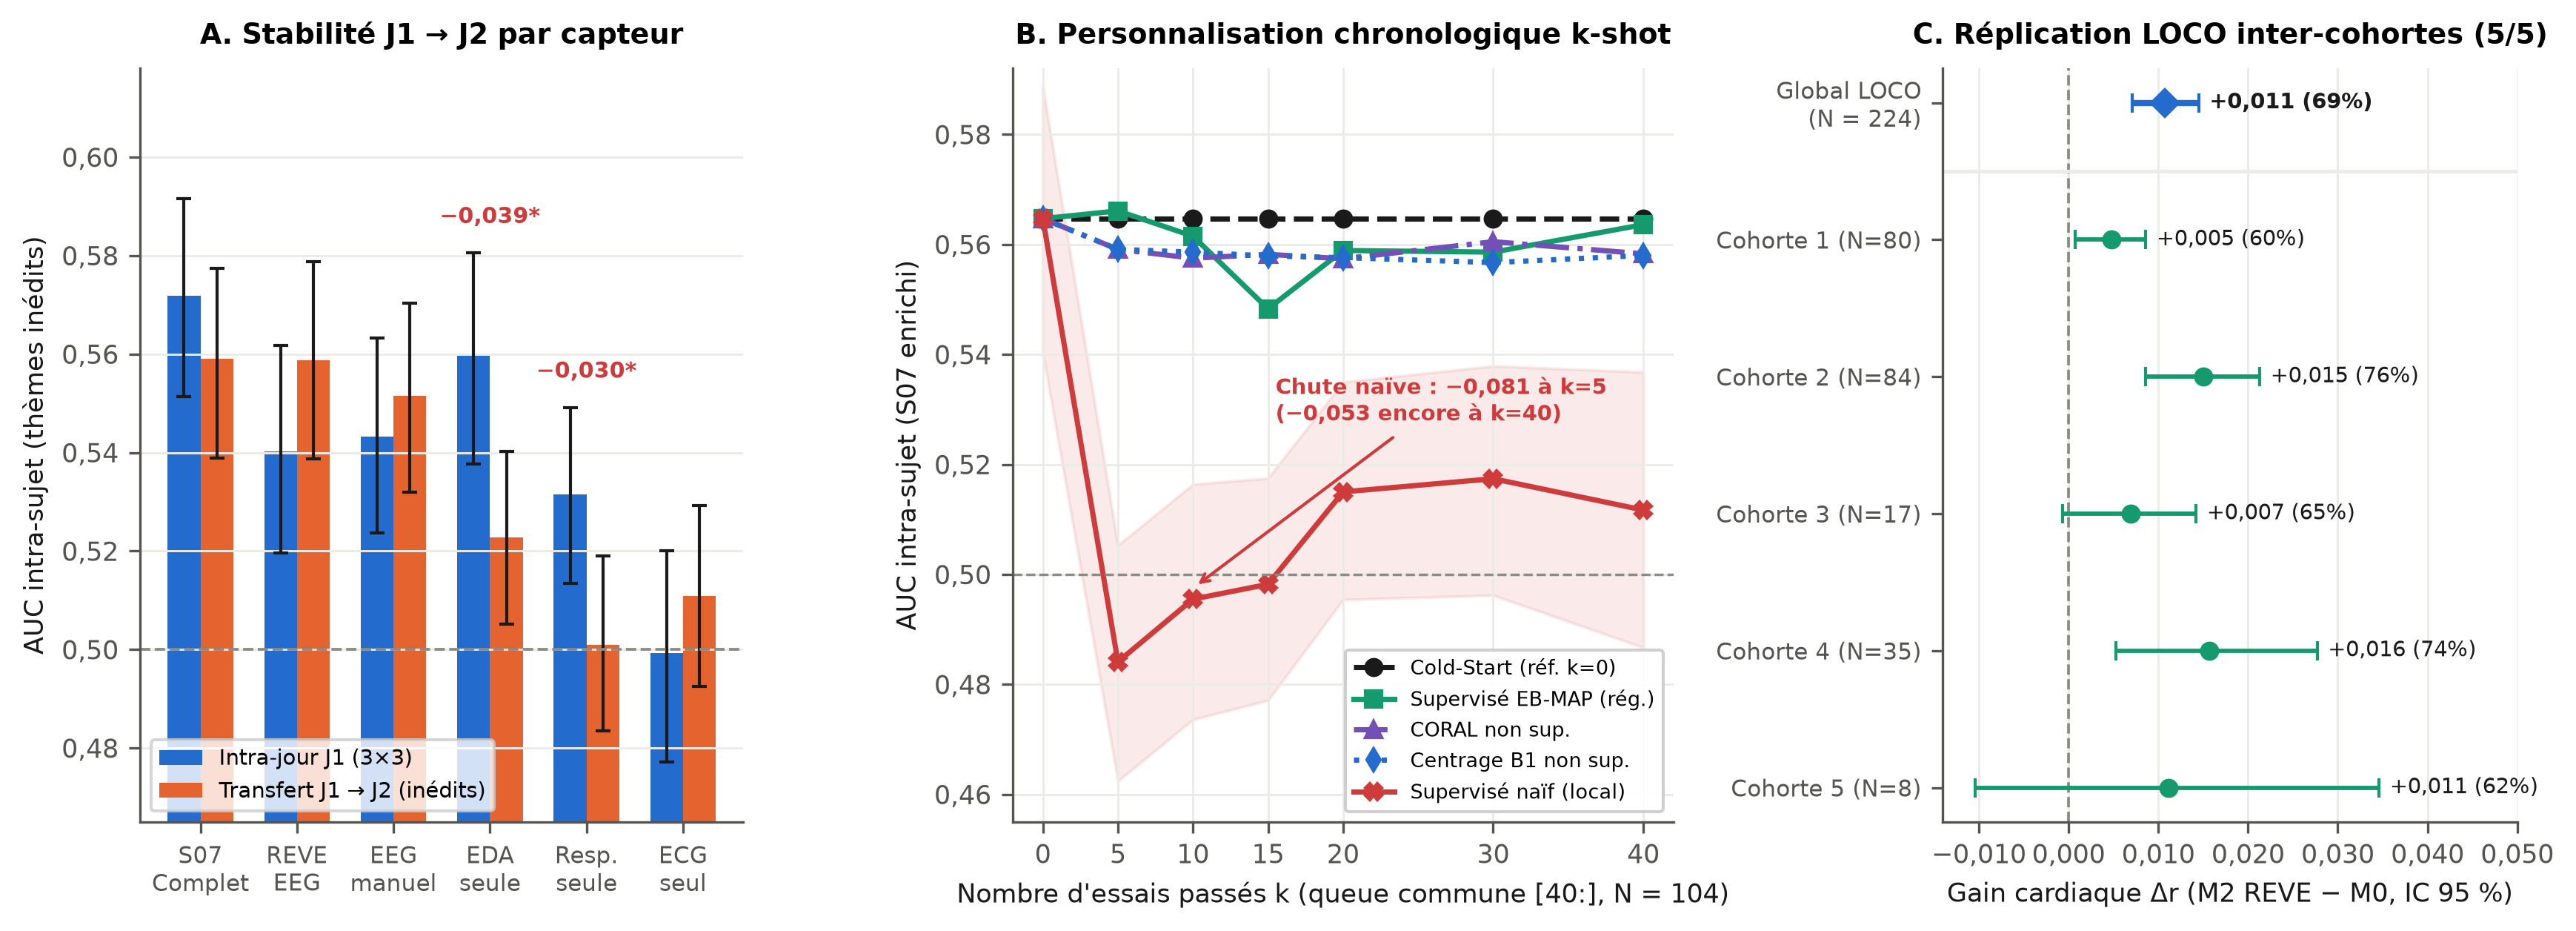
\includegraphics[width=0.98\linewidth]{fig2_longitudinal_personalization_fr.png}
\caption{\textbf{Stabilité inter-jours J1 $\to$ J2, personnalisation chronologique $k$-shot et réplication LOCO (Études 10B--C).} \textbf{A.} Transfert d'un décodeur entraîné sur J1 et testé sur J2 (thèmes inédits) : chute significative de l'EDA ($-0{,}039^*$) et de la respiration ($-0{,}030^*$), stabilité de l'EEG et du multimodal. \textbf{B.} Courbe $k$-shot ($k = 0 \dots 40$, queue commune \texttt{[40:]}, $N = 104$) : effondrement massif de la personnalisation supervisée naïve, neutralisé par le \emph{shrinkage} bayésien EB-MAP. \textbf{C.} Réplication hors-cohorte LOCO du gain cardiaque \texttt{M2 $-$ M0} dans 5/5 cohortes.}
\label{fig:longit}
\end{figure}

L'analyse des 169 participants multi-jours (121 en \texttt{dev}) et des terciles chronologiques intra-session (figure~\ref{fig:longit} et tableau~\ref{tab:study10_gen}) confirme et précise quatre hypothèses majeures de la revue de littérature :
\begin{enumerate}
\item \textbf{Dérive inter-jours de l'EDA (Sakimura et al.\ \cite{sakimura2025}) :} l'EDA présente la plus faible stabilité tonique de repos d'un jour à l'autre ($r = 0{,}420$ [$0{,}226 ; 0{,}585$] contre $0{,}569$ ECG, $0{,}707$ Resp, $0{,}724$ alpha occipital et $0{,}664$ taux de stress). Surtout, en transfert de décodeur \texttt{J1 $\to$ J2} sur thèmes inédits (figure~\ref{fig:longit}A), \textbf{\texttt{EDA\_only} chute significativement de $0{,}5597$ à $0{,}5228$ ($-0{,}0392$ [$-0{,}0728 ; -0{,}0085$])}, tout comme \texttt{Resp\_only} ($0{,}5315 \to 0{,}5010$, $-0{,}0299^*$), tandis que \texttt{EEG\_hc\_only} ($0{,}543 \to 0{,}552$), \texttt{REVE\_frozen} ($0{,}540 \to 0{,}559$) et le multimodal \texttt{S07} ($0{,}572 \to 0{,}559$ nouveaux sujets, $0{,}567$ mêmes sujets) demeurent stables. La répétabilité individuelle des pentes de réactivité $r(\rho_{J1}, \rho_{J2})$ est modérée et comparable entre capteurs ($0{,}21$--$0{,}26$ pour FC, RR, delta, EDA et pupille).
\item \textbf{Habituation intra-session dissociée (Chen et al.\ \cite{chen2014}) :} ajustés sur le consensus vidéo ($N = 314$), les pics électrodermaux \texttt{SCR} s'habituent au fil de la session ($\rho_{\text{rang}} = -0{,}0322$ [$-0{,}0535 ; -0{,}0106$]), alors que le freinage vagal cardiaque ne s'habitue pas ($\Delta\mathrm{RR}_{T3-T1} = +5{,}66$~ms [$+0{,}12 ; +11{,}62$]) et que la suppression alpha occipitale s'accentue ($-0{,}0710$ [$-0{,}090 ; -0{,}052$]).
\item \textbf{Effondrement de la personnalisation supervisée naïve (Khan \& Ishikawa \cite{khan2026}) :} sur la queue future commune \texttt{[40:]} ($N = 104$, 4\,203 essais, figure~\ref{fig:longit}B), un modèle supervisé personnel naïf entraîné sur $k$ essais labellisés du sujet s'effondre catastrophiquement sous le Cold-Start ($0{,}5647$) : \textbf{$0{,}4841$ ($-0{,}0806$) à $k = 5$}, $0{,}4955$ à $k = 10$, $0{,}5150$ à $k = 20$ et encore \textbf{$0{,}5117$ ($-0{,}0530$) à $k = 40$} (et $-0{,}0401^*$ sur S07 / $-0{,}0686^*$ sur REVE en calibration complète \texttt{J1 $\to$ J2}, $N = 108$). Notre adaptation bayésienne empirique (\texttt{EB-MAP} centrée sur $w_{\text{pop}}$) élimine totalement la chute ($0{,}5661$ à $k = 5$, $0{,}5636$ à $k = 40$ ; jusqu'à $+0{,}0104$ à $k = 15$ sur \texttt{REVE}) mais démontre honnêtement que quelques dizaines d'essais ne suffisent pas à débloquer un gain individuel massif.
\item \textbf{Transfert inter-cohortes LOCO et CORAL (Mihirette et al.\ \cite{mihirette2025}) :} sur les 5 cohortes évaluées hors-cohorte en \texttt{dev}, le détecteur multimodal transfère nativement à \textbf{0,5893} [$0{,}574 ; 0{,}605$] ($0{,}575$--$0{,}604$ selon les cohortes ; \texttt{REVE} $0{,}5612$). L'alignement non supervisé CORAL reste neutre en AUC intra ($-0{,}0009$ S07, $-0{,}0006$ REVE ; léger gain poolé $0{,}5674 \to 0{,}5702$ et sur la petite cohorte 5 en REVE $0{,}547 \to 0{,}576$) car les cinq cohortes partagent déjà le même protocole matériel et le référencement pré-stimulus par essai.
\end{enumerate}

\begin{table}[t]
\centering\scriptsize\setlength{\tabcolsep}{3.5pt}
\begin{tabular}{@{}llrrr@{}}
\toprule
Expérience (Étude 10A--C) & Condition / Capteur & AUC ou $r$ & Gain apparié vs réf. & $N$\\
\midrule
Échelle \texttt{S07} V\&A & R1 / R3 / R2 / \textbf{R4 strict} & 0,589 / 0,583 / 0,573 / \textbf{0,569} & $\text{R1}-\text{R4} = +0{,}020$ & 208\\
Ablation R4 Cold-Start & \texttt{-EEG} / \texttt{-EDA} / \texttt{-ECG} / \texttt{ECG seul} & 0,540 / 0,551 / 0,569 / 0,508 & $\mathbf{-0{,}028^*}$ / $\mathbf{-0{,}018^*}$ / $0{,}000$ & 208\\
\midrule
Transfert \texttt{J1 $\to$ J2} & \texttt{EDA\_only} / \texttt{Resp\_only} & $0{,}560 \to 0{,}523$ ; $0{,}532 \to 0{,}501$ & $\mathbf{-0{,}039^*}$ / $\mathbf{-0{,}030^*}$ & 108\\
 & \texttt{EEG\_hc} / \texttt{REVE} / \texttt{S07 complet} & $0{,}552$ / $0{,}559$ / $0{,}559$ & $+0{,}025$ / $+0{,}015$ / $+0{,}004$ & 108\\
\midrule
$k$-shot \texttt{S07} (\texttt{[40:]}) & CS / Naïf ($k=10, 40$) / EB-MAP & 0,565 / 0,496--0,512 / 0,564 & Naïf $\mathbf{-0{,}069}$ à $\mathbf{-0{,}053}$ & 104\\
Calibration \texttt{J1 $\to$ J2} & \texttt{S07} / \texttt{REVE} : Naïf vs EB-MAP/CORAL & 0,524 / 0,496 vs 0,563--0,569 & Naïf $\mathbf{-0{,}040^*}$ / $\mathbf{-0{,}069^*}$ & 108\\
\midrule
LOCO inter-cohortes & Stress \texttt{S07} / \texttt{REVE} (brut vs CORAL) & 0,589/0,588 ; 0,561/0,561 & $-0{,}001$ / $-0{,}001$ (neutre) & 208\\
 & \textbf{ECG \texttt{M2 $-$ M0} LOCO (5/5 cohortes)} & $0{,}6885 \to \mathbf{0{,}6992}$ & $\mathbf{+0{,}0107^*}$ [$+0{,}007 ; +0{,}015$] & 224\\
\bottomrule
\end{tabular}
\caption{Synthèse des résultats de généralisation, stabilité longitudinale, personnalisation et transfert LOCO (Étude 10A--C).}
\label{tab:study10_gen}
\end{table}

\section{Cohérence autonome--subjective et monitoring clinique passif (Étude 10D--E)}
\label{sec:clinical}

\subsection{Orthogonalité autonome--subjective et hétérogénéité individuelle sur 314 personnes}

\begin{figure}[t]
\centering
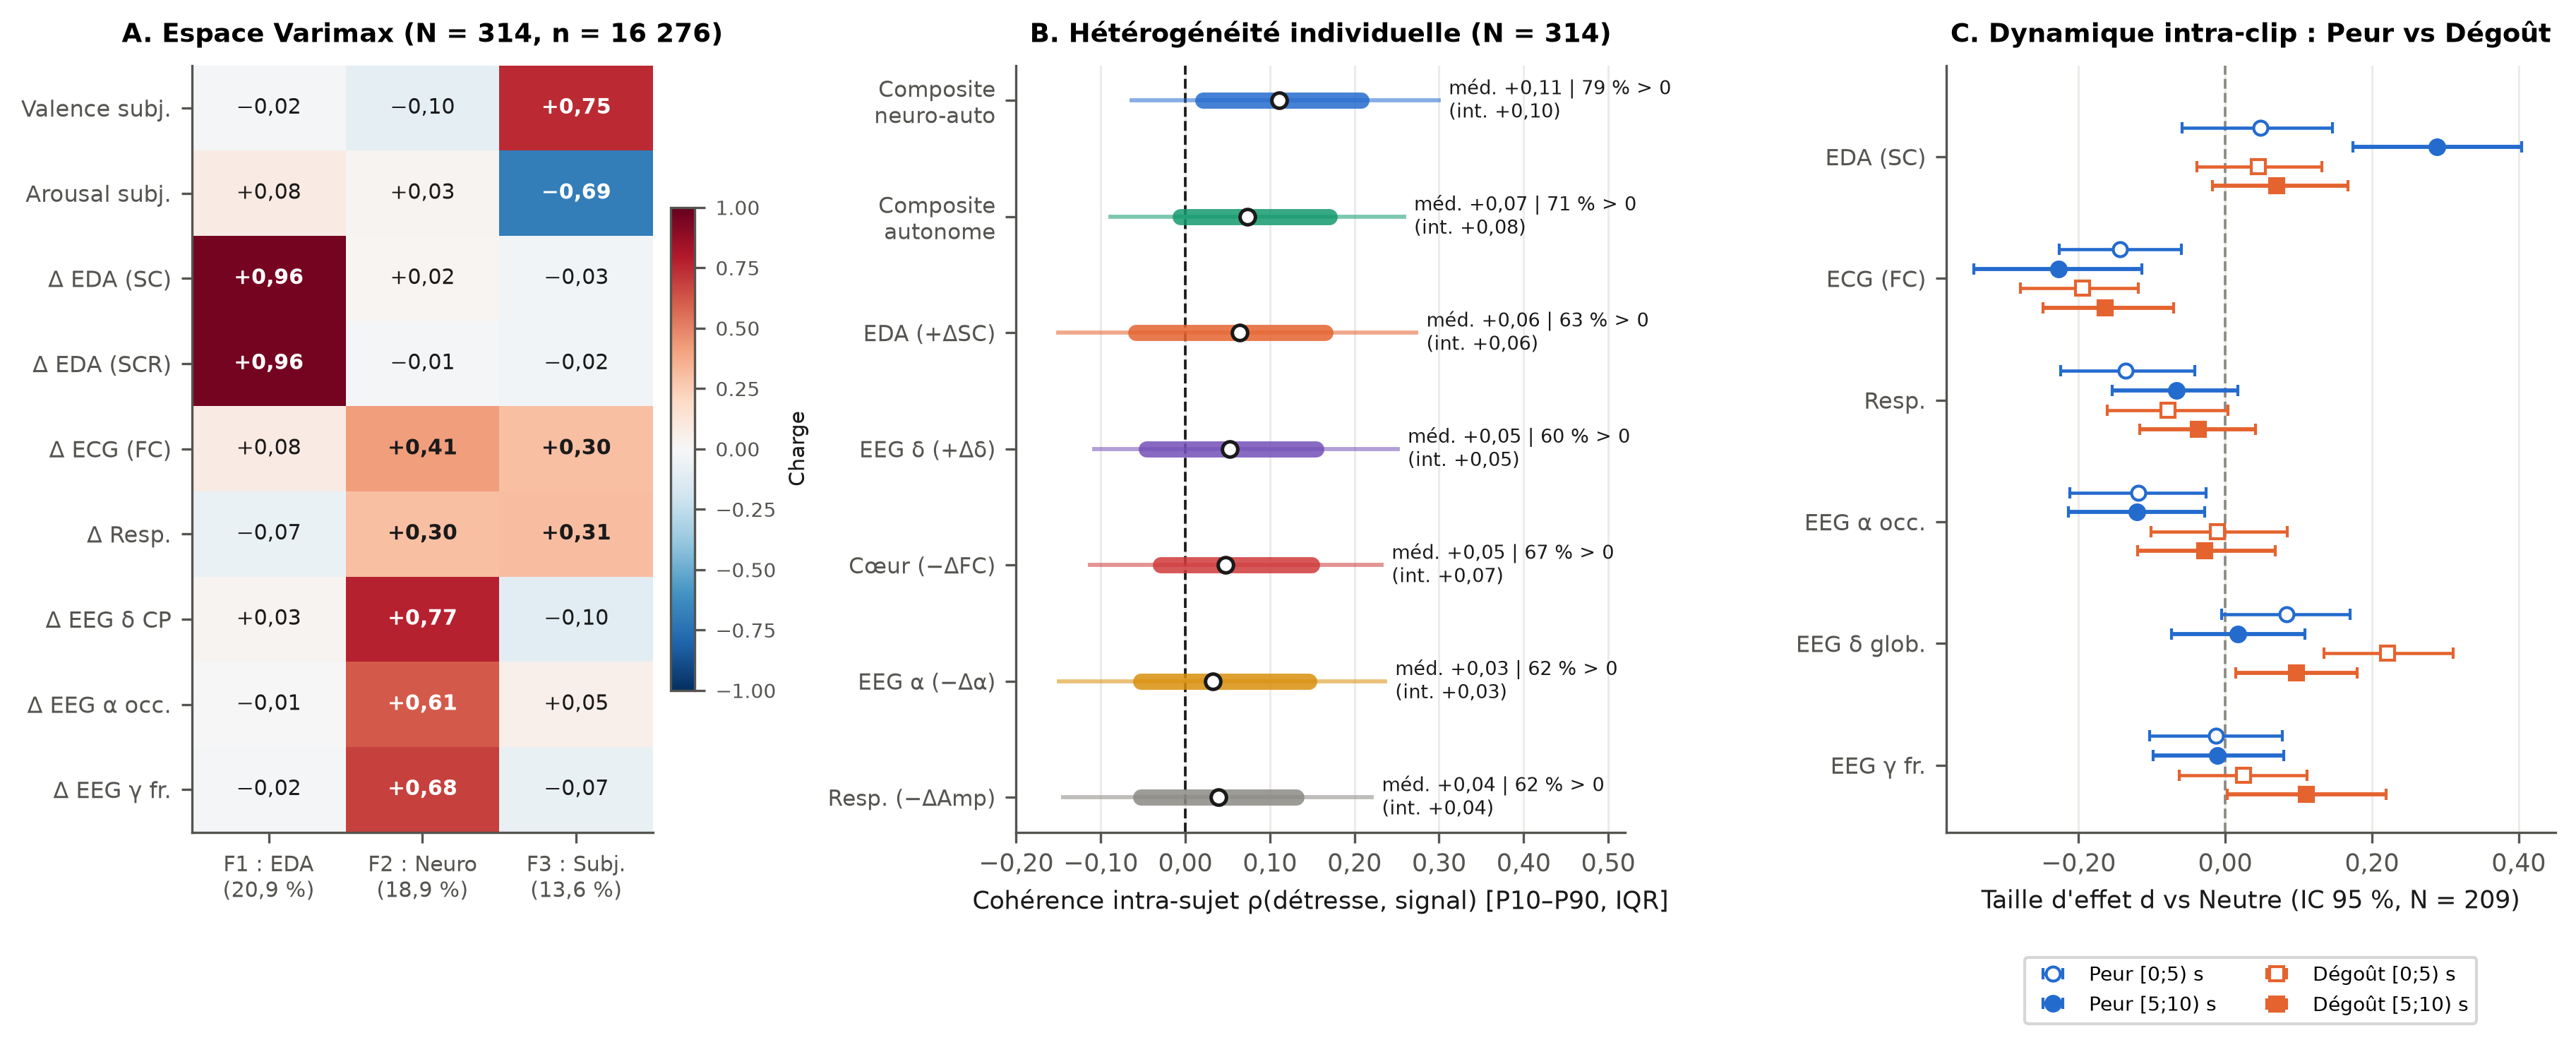
\includegraphics[width=0.98\linewidth]{fig3_coherence_withinclip_fr.png}
\caption{\textbf{Cohérence autonome--subjective ($N = 314$) et dynamique intra-clip Peur vs Dégoût ($N = 209$) (Étude 10D et 10F).} \textbf{A.} Charges factorielles Varimax à 3 dimensions ($n = 16\,276$) répliquant à $6\times$ l'échelle la divergence de Cuve et al.\ \cite{cuve2023}. \textbf{B.} Distribution individuelle (P10--P90, IQR, médiane, \% $> 0$ et gain d'intensité) répliquant Brown et al.\ \cite{brown2019}. \textbf{C.} Effets intra-clip précoces $[0 ; 5)$~s (creux) vs tardifs $[5 ; 10)$~s (pleins) de la peur et du dégoût contre neutre.}
\label{fig:coh_wclip}
\end{figure}

L'analyse de l'espace affectif sur l'ensemble des 314 participants ($n = 16\,276$ essais complets, figure~\ref{fig:coh_wclip}A) réplique à six fois l'échelle le résultat fondateur de Cuve et al.\ \cite{cuve2023} ($N = 51$) et l'étend à l'EEG cortical. Les trois facteurs Varimax (53,3\,\% de la variance intra-sujet) séparent rigoureusement : (i)~\textbf{F1 (20,9\,\%)}, un axe sympathique électrodermal quasi pur ($\Delta\text{SC} = +0{,}96$, $\Delta\text{SCR} = +0{,}96$, arousal $+0{,}08$) ; (ii)~\textbf{F2 (18,9\,\%)}, un axe de covariance neuro-cardio-respiratoire ($\Delta\delta_{\text{CP}} +0{,}77$, $\Delta\gamma_{\text{fr}} +0{,}68$, $\Delta\alpha_{\text{occ}} +0{,}61$, $\Delta\text{FC} +0{,}41$, $\Delta\text{Resp} +0{,}30$) \textbf{quasi orthogonal au ressenti subjectif} (valence $-0{,}10$, arousal $+0{,}03$) ; et (iii)~\textbf{F3 (13,6\,\%)}, l'axe partagé de cohérence subjective--cardio-respiratoire (valence $+0{,}75$, arousal $-0{,}69$, $\Delta\text{FC} +0{,}30$, $\Delta\text{Resp} +0{,}31$). Cette structure survit intégralement après résidualisation sur la vidéo (part idiosyncrasique). Elle fournit la raison biophysique directe pour laquelle les AUC sur essai unique plafonnent autour de $0{,}57$--$0{,}60$ malgré des modèles à 69~M paramètres : une part substantielle de la variance autonome et corticale ne covarie tout simplement pas avec la note verbale.

Au niveau individuel (figure~\ref{fig:coh_wclip}B), nos 314 sujets répliquent à cinq fois l'échelle Brown et al.\ \cite{brown2019} ($N = 63$) et les modèles de variabilité de réactivité \cite{nguyen2026,maxwell2018,saviola2020,sato2020} : chaque capteur isolé affiche une cohérence intra-personne $\rho_i$ modeste et très dispersée ($+0{,}040$ à $+0{,}060$, 60--67\,\% positifs), mais le \textbf{composite neuro-autonome double la cohérence} (moyenne $+0{,}1155$ [$+0{,}099 ; +0{,}131$], médiane $+0{,}111$, IQR $[+0{,}021 ; +0{,}208]$, P10--P90 $[-0{,}064 ; +0{,}300]$), révélant \textbf{79,0\,\% d'individus cohérents ($> 0$)}, 26,8\,\% fortement cohérents ($> 0{,}20$) et \textbf{21,0\,\% discordants ($< 0$)}. Surtout, l'effet d'intensité émotionnelle prédit par Brown et al.\ \cite{brown2019} est massif : comparer les essais d'intensité extrême aux essais modérés élève la cohérence de \textbf{$+0{,}1008$} [$+0{,}074 ; +0{,}129$] sur le composite neuro-autonome ($+0{,}067^*$ sur le cœur, $+0{,}060^*$ sur l'EDA), et la cohérence cardiaque ($r_{J1,J2} = 0{,}237^*$), delta ($0{,}215^*$) et EDA ($0{,}197^*$) montre une composante trait partiellement stable d'un jour à l'autre. Enfin, le pont avec l'Étude~09 ($N = 224$) montre que le gain individuel d'anticipation cerveau--cœur $\Delta r_i = r_i(\text{M2}) - r_i(\text{M0})$ est indépendant du taux de stress trait ($\rho = -0{,}057$), de la FC basale ($+0{,}077$), de la réactivité cardiaque ($+0{,}004$) et de la cohérence subjective ($\rho = +0{,}091$, $p = 0{,}177$) : il reflète un couplage neuroviscéral général présent même chez les sujets subjectivement peu cohérents.

\subsection{Simulation opérationnelle de monitoring clinique passif (10 s à 100 s)}

\begin{figure}[t]
\centering
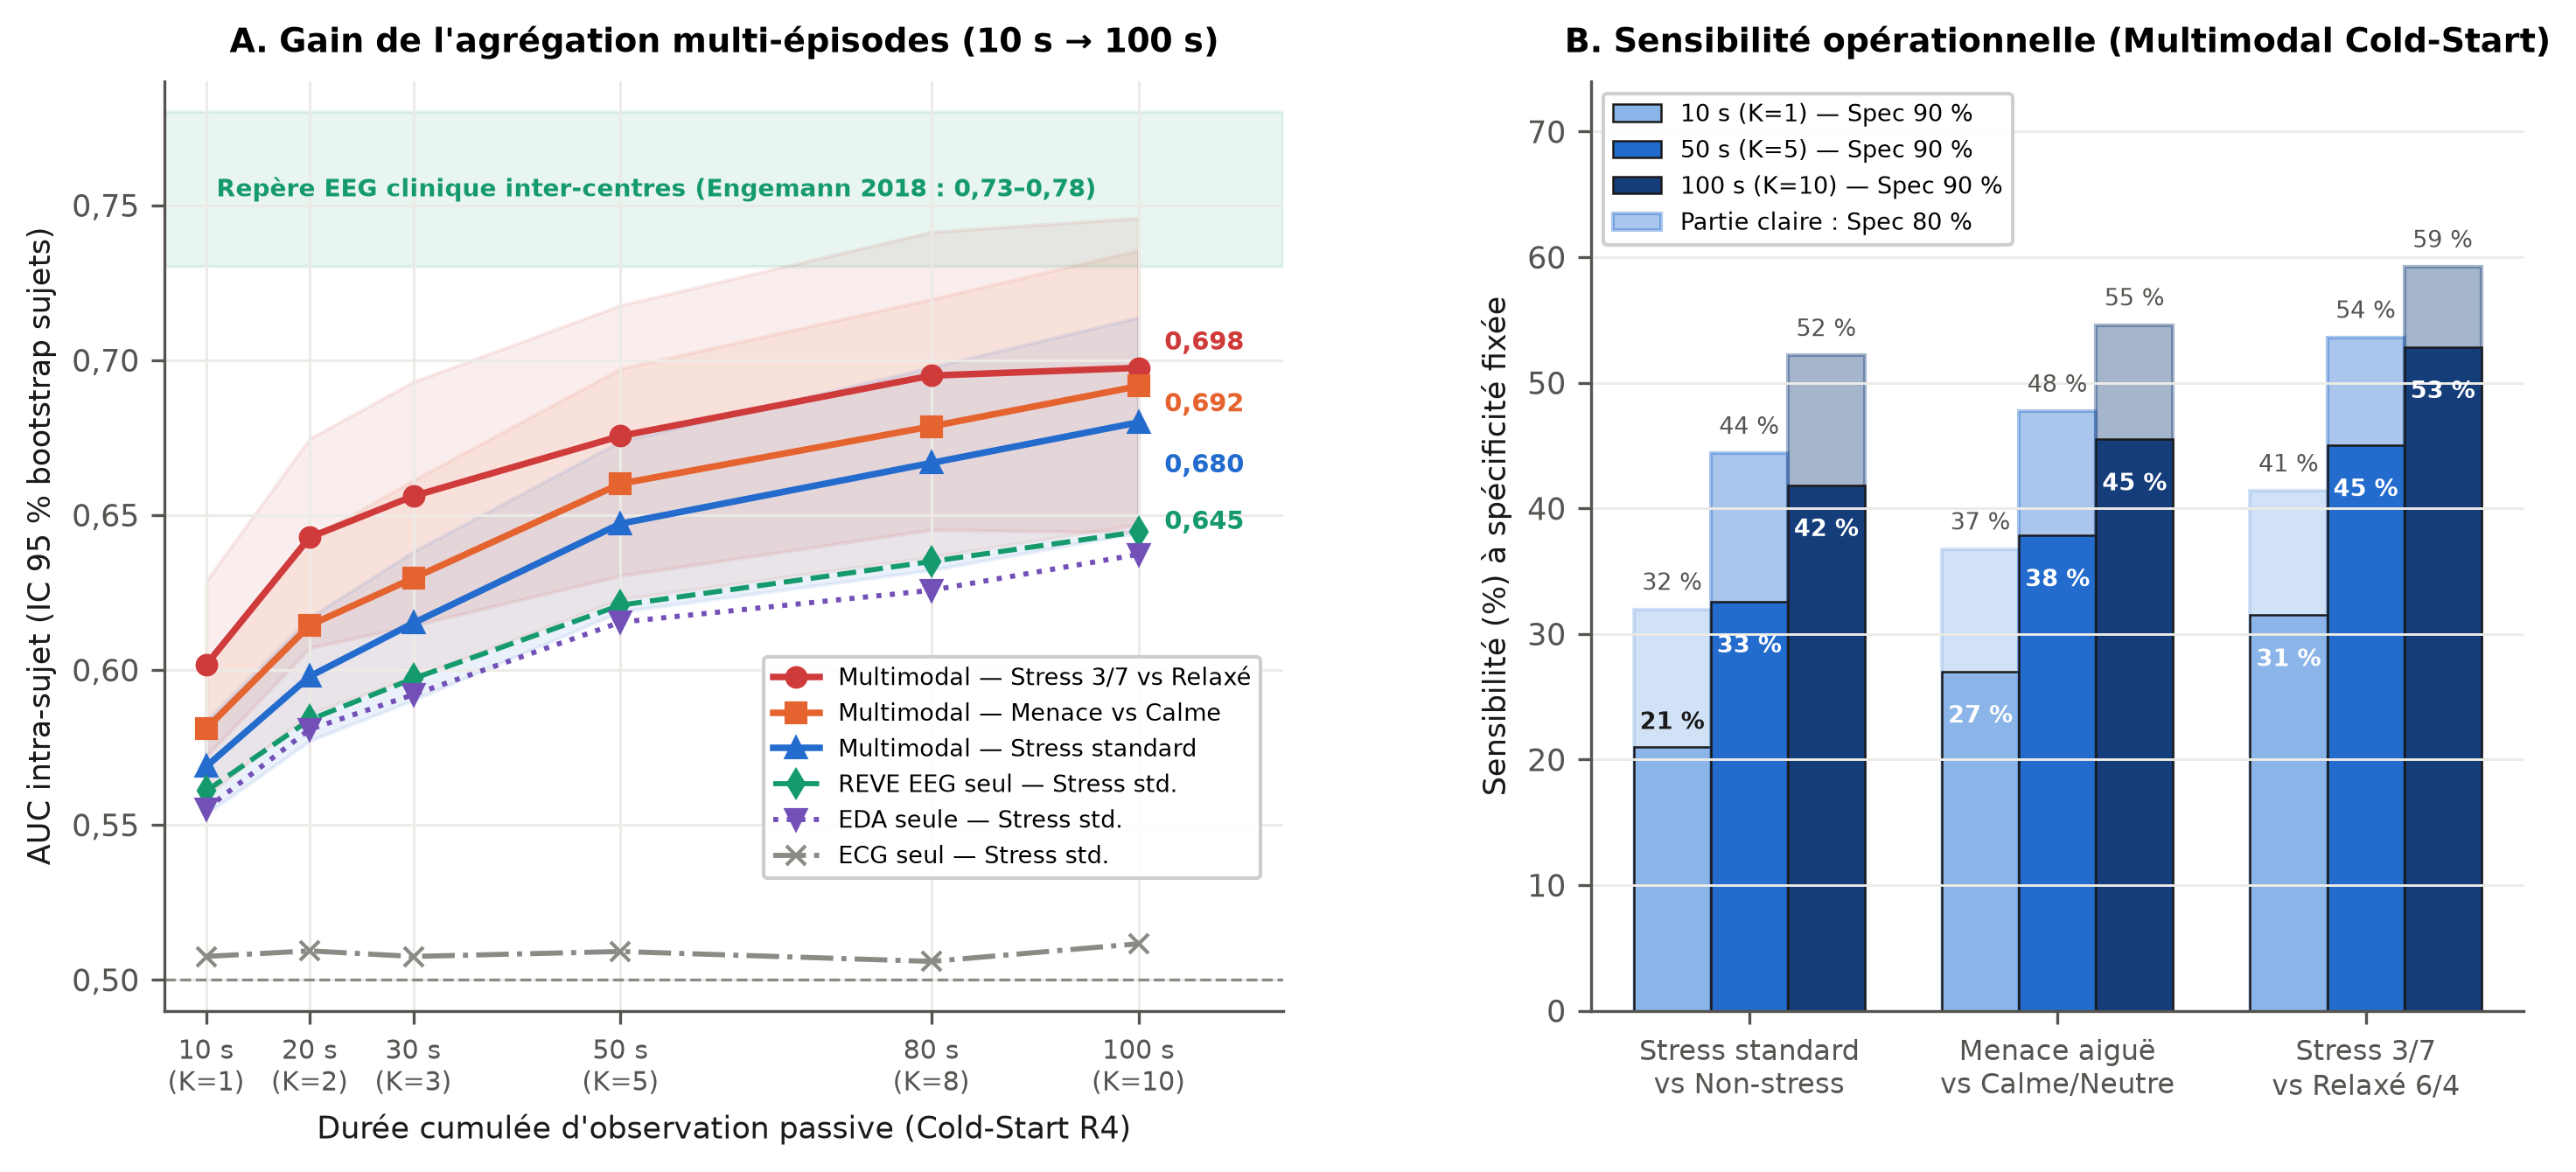
\includegraphics[width=0.98\linewidth]{fig4_clinical_monitoring_fr.png}
\caption{\textbf{Simulation opérationnelle de monitoring clinique passif multi-épisodes en Cold-Start strict (Étude 10E, \texttt{dev}).} \textbf{A.} Progression monotone de l'AUC intra-sujet de $K = 1$ (10~s) à $K = 10$ épisodes (100~s) pour trois contrastes cliniques et quatre modalités, comparée au repère EEG clinique inter-centres d'Engemann et al.\ \cite{engemann2018}. \textbf{B.} Sensibilité opérationnelle à 80\,\% et 90\,\% de spécificité pour le détecteur multimodal à 10~s, 50~s et 100~s.}
\label{fig:clinical}
\end{figure}

Pour traduire nos mesures en bornes cliniques concrètes (figure~\ref{fig:clinical}), nous simulons sur les prédictions strictement Cold-Start R4 l'agrégation de $K = 1$ à $10$ épisodes de 10~s (soit 10~s à 100~s d'observation passive, vérifiée par tirages strictement sans remise à $K = 3$ et $5$). L'agrégation temporelle produit un gain monotone de $+0{,}10$ à $+0{,}11$ AUC sur les trois contrastes :
\begin{itemize}
\item \textbf{Stress standard vs Non-stress ($N = 208$) :} AUC de $0{,}5688$ (10~s) à $0{,}6472$ (50~s ; sans remise $0{,}6344$) et \textbf{0,6799} (100~s), doublant la sensibilité à 90\,\% de spécificité (\textbf{21\,\% $\to$ 42\,\%}, et 52\,\% à 80\,\% de spécificité).
\item \textbf{Menace aiguë (peur/colère/dégoût) vs Calme/Neutre ($N = 139$) :} AUC de $0{,}5810$ (10~s) à $0{,}6601$ (50~s ; sans remise \textbf{0,6958}) et \textbf{0,6916} (100~s), sensibilité à 90\,\% de spécificité de 27\,\% à \textbf{45\,\%} (55\,\% à 80\,\%).
\item \textbf{Stress aigu franc ($V\le 3, A\ge 7$) vs Calme/Relaxé ($V\ge 6, A\le 4$) ($N = 147$) :} AUC de $0{,}6016$ (10~s) à \textbf{0,6975} (100~s), sensibilité à 90\,\% de spécificité de 31\,\% à \textbf{53\,\%} (59\,\% à 80\,\%).
\end{itemize}
À 100~s, le détecteur multimodal ($0{,}680$--$0{,}698$) devance nettement chaque capteur seul (\texttt{REVE} EEG $0{,}594$--$0{,}645$, \texttt{EDA} $0{,}637$--$0{,}693$, \texttt{EEG manuel} $0{,}621$--$0{,}633$, \texttt{ECG} $0{,}512$--$0{,}539$).

\section{Discussion, transposition clinique, limites et reproductibilité}
\label{sec:discussion}

\begin{table}[t]
\centering\footnotesize
\begin{tabularx}{\linewidth}{@{}L{2.5cm} Y L{4.7cm}@{}}
\toprule
Axe scientifique & Conclusion établie (Études 04--10) & Portée méthodologique / clinique\\
\midrule
Architecture du stress (É05--07, 10F) & 3 branches : $\alpha$ occipitale automatique, bradycardie vagale sinusale évaluative (PR nul), alarme EDA/$\delta$ à seuil haut ; peur $\neq$ dégoût. & Ne pas supposer une tachycardie linéaire ni utiliser RMSSD/Bazett/HEP sur 10~s.\\
Prévision EEG $\to$ Corps (É09, 10C) & Gain cardiaque causal réel, idiosyncrasique, résistant aux artefacts, répliqué dans 5/5 cohortes LOCO ; réfuté sur EDA et Resp. & Mur causal matériel obligatoire ; contrôle non linéaire \texttt{M0\_gbdt} indispensable.\\
Modèles \& généralisation (É08--10C) & 4 phases linéaires 0-GPU égalent ou battent FMs/JEPA/LoRA/stacking ; R1/R3 gonflent ; EDA dérive J1$\to$J2 ; naïf $k$-shot échoue. & Évaluer en R4 double inédit ; combiner EEG + EDA ; proscrire la calibration naïve $<40$ essais.\\
Cohérence \& clinique (É10D--E) & 3 axes orthogonaux (Cuve) ; 79\,\% cohérents, 21\,\% discordants (Brown) ; agrégation 100~s $\to$ AUC 0,68--0,70 (Spec90 : 42--53\,\%). & Monitoring passif = indicateur de tendance agrégé ($\ge 1$--$2$~min), jamais verdict sur 10~s.\\
\bottomrule
\end{tabularx}
\caption{Synthèse générale des acquis scientifiques et des règles opérationnelles de l'Équipe 12.}
\label{tab:final_synthesis}
\end{table}

\paragraph{Ce que nous apportons à la littérature.}
Réunis dans le tableau~\ref{tab:final_synthesis}, nos résultats apportent quatre contributions empiriques à une échelle (314 sujets, 22\,974 essais) rarement égalée en psychophysiologie affective. Premièrement, nous unifions la physiologie du stress aigu bref autour d'une dissociation à trois étages — réflexe attentionnel alpha \cite{codispoti2023,stegmann2024}, freinage vagal sinusal pur sans composante nodale PR \cite{somsen2002,abercrombie2008}, et alarme sympathique/corticale à seuil élevé avec dynamique intra-clip spécifique par émotion \cite{si2026,qin2023}. Deuxièmement, nous démontrons sous mur causal strict et 12 contrôles qu'une information EEG précoce idiosyncrasique anticipe réellement la trajectoire cardiaque future au-delà du passé corporel (y compris en LOCO sur 5/5 cohortes), tout en réfutant la même hypothèse sur l'EDA et la respiration. Troisièmement, nous expliquons pourquoi l'augmentation de capacité algorithmique (jusqu'à 69,2~M paramètres et LoRA) échoue à déplacer le score de stress subjectif : la majeure partie de la variance autonome--corticale est orthogonale aux notes subjectives \cite{cuve2023}, 21\,\% des sujets sont discordants \cite{brown2019}, l'EDA dérive d'un jour à l'autre \cite{sakimura2025} et une personnalisation naïve sur peu d'essais sur-ajuste massivement \cite{khan2026}.

\paragraph{Transposition réaliste au monitoring clinique non verbal.}
Nos courbes d'agrégation passive éclairent directement la faisabilité clinique discutée par Engemann et al.\ \cite{engemann2018}, Roué et al.\ \cite{roue2025}, Adama \& Bogdan \cite{adama2025}, Danel et al.\ \cite{danel2025} et Paniagua-Gómez \& Fernandez-Carmona \cite{paniagua2025}. D'une part, agréger 50 à 100~s d'observation multimodale sans aucune étiquette du patient élève l'AUC Cold-Start jusqu'à $0{,}68$--$0{,}70$ (sensibilité 53--59\,\% à 80--90\,\% de spécificité sur les états francs), approchant le plancher de généralisation EEG clinique inter-centres ($0{,}73$--$0{,}78$ \cite{engemann2018}). D'autre part, ce niveau demeure inférieur aux $0{,}90$ rapportés en douleur procédurale néonatale \cite{roue2025}, pour deux raisons biologiques claires : des vidéos passives de 10~s n'induisent ni nociception somatique ni stress prolongé, et la divergence autonome--subjective limite structurellement la correspondance essai par essai. En pratique clinique (réanimation, anesthésie, patients non communicants), un moniteur multimodal EEG + EDA doit donc opérer comme un \textbf{indicateur probabiliste agrégé sur au moins 1 à 2 minutes}, recalibré de façon bayésienne pour compenser la dérive inter-jours de l'EDA, et toujours interprété dans son contexte pharmacologique et clinique \cite{danel2025}.

\paragraph{Discipline épistémique, limites et reproductibilité.}
Nous maintenons une frontière stricte entre \emph{prédiction temporelle incrémentale}, \emph{association} et \emph{causalité mécanistique} : le gain cardiaque \texttt{M2 $-$ M0} établit une prévisibilité conditionnelle au sens de Granger, non une causalité descendante directe (un état sous-cortical non mesuré pouvant précéder simultanément l'EEG et le cœur). Nos conclusions valent conditionnellement à des clips passifs de 10~s chez l'adulte sain, sans douleur physique, sans dérivation ECG multiple, et avec une contribution micro-EMG faciale résiduelle possible sur le gamma frontal (notamment dans le dégoût tardif). Nous ne revendiquons aucun plafond physiologique absolu. L'intégralité des scripts (\texttt{decoding/\allowbreak rich\_extract.py}, \texttt{revision.py}, \texttt{ssl\_*.py}, \texttt{study09\_*.py}, \texttt{study10\_final.py}), des protocoles pré-enregistrés (\texttt{journal/\allowbreak 04..10*.md}), des tests unitaires, des agrégats JSON publics et des scripts de figures est versionnée et reproductible dans le dépôt sans qu'aucune donnée individuelle ne quitte les serveurs HABS.

\begin{otherlanguage*}{english}
\begin{thebibliography}{99}\footnotesize\setlength{\itemsep}{1.0pt}
% Axe 1: Réponses autonomes rapides (9)
\bibitem{abercrombie2008} H. C. Abercrombie et al. Orienting, emotion, and memory: phasic and tonic variation in heart rate predicts memory for emotional pictures in men. Neurobiol. Learn. Mem. 90 (2008) 644--650.
\bibitem{jennings1980} J. R. Jennings, D. Schrot, C. C. Wood. Cardiovascular response patterns during choice reaction time. Physiol. Psychol. 8 (1980) 127--133.
\bibitem{somsen2002} R. J. M. Somsen, J. R. Jennings, M. W. van der Molen. Human vagal heart rate responses in warned reaction time tasks: a cross-validation with simulated vagus--sino-atrial node interactions. J. Electrocardiol. 35 (2002) 131--138.
\bibitem{chen2014} K. H. Chen et al. Habituation of parasympathetic-mediated heart rate responses to recurring acoustic startle. Front. Psychol. 5 (2014) 1288.
\bibitem{coelli2026} S. Coelli et al. Modulation of autonomic responses to cognitive tasks under acute mental stress. Sci. Rep. (2026) doi:10.1038/s41598-025-34921-4.
\bibitem{schippers2018} A. Schippers et al. Ultra-short term heart rate variability as a tool to assess changes in valence. Psychiatry Res. 270 (2018) 517--522.
\bibitem{sakimura2025} M. Sakimura et al. Long-term variability in physiological-arousal relationships for robust emotion estimation. ACII 2025, arXiv:2508.18782.
\bibitem{qin2023} X. Qin et al. Different affective arousal and adaptation pattern between core and moral disgust: evidence from subjective emotional experience and autonomic nervous system activity. J. Psychol. Sci. 46 (2023) 320--328.
\bibitem{collet1997} C. Collet, E. Vernet-Maury, G. Delhomme, A. Dittmar. Autonomic nervous system response patterns specificity to basic emotions. J. Auton. Nerv. Syst. 62 (1997) 45--57.
% Axe 2: Décalage EEG/SNA, généralisation & adaptation de domaine (9)
\bibitem{hinduja2023} S. Hinduja et al. Multimodal temporal modeling of emotion using physiological signals. ACII 2023, TechRxiv:23548131.
\bibitem{liu2021} S. Liu et al. EEG-based multimodal emotion recognition: a machine learning perspective. Aalborg Univ. (2021).
\bibitem{engemann2018} D. A. Engemann et al. Robust EEG-based cross-site and cross-protocol classification of states of consciousness. Brain 141 (2018) 3179--3192.
\bibitem{alshamrani2026} M. Alshamrani. Cross-subject generalization in wearable physiological monitoring: real-time four-class state classification using multimodal machine learning. J. Eng. Res. (2026) S2307187726001586.
\bibitem{mihirette2025} A. Mihirette et al. Cross-contextual stress prediction: simple methodology for comparing features and sample domain adaptation. Appl. Intell. 55 (2025) doi:10.1007/s10489-025-06277-9.
\bibitem{si2026} Y. Si et al. Time-resolved EEG characteristics track within-clip emotion dynamics. SSRN Preprint (2026).
\bibitem{jomaa2026} R. Jomaa et al. Real-time cross-subject emotional arousal estimation in virtual reality using low-density EEG: a multimodal physiological validation. Biomed. Signal Process. Control (2026) S1746809426015739.
\bibitem{alasfour2025} A. Alasfour, M. AlSabah. EEG-based prediction of stress responses to naturalistic decision-making stimuli in police cadets. Sensors 25 (2025) 5925.
\bibitem{jeong2026} H. Jeong et al. Time-resolved EEG decoding reveals altered neural dynamics of affective semantic evaluation in depression and suicidality. Commun. Biol. (2026) doi:10.1038/s42003-026-10108-z.
% Axe 3: EEG, attention & limites inter-sujets (11)
\bibitem{codispoti2023} M. Codispoti, A. De Cesarei, V. Ferrari. Alpha-band oscillations and emotion: a review of studies on picture perception. Psychophysiology 60 (2023) e14438.
\bibitem{stegmann2024} Y. Stegmann et al. Electrocortical responses in anticipation of avoidable and inevitable threats: a multisite study. J. Neurosci. 44 (2024) PMC11484543.
\bibitem{panitz2019} C. Panitz, A. Keil, E. M. Mueller. Extinction-resistant attention to long-term conditioned threat is indexed by selective visuocortical alpha suppression in humans. Sci. Rep. 9 (2019) 15809.
\bibitem{zumer2014} J. M. Zumer et al. Occipital alpha activity during stimulus processing gates the information flow to object-selective cortex. PLOS Biol. 12 (2014) e1001965.
\bibitem{bacigalupo2022} F. Bacigalupo, S. J. Luck. Alpha-band EEG suppression as a neural marker of sustained attentional engagement to conditioned threat stimuli. Soc. Cogn. Affect. Neurosci. 17 (2022) 1101--1117.
\bibitem{simons2009} R. F. Simons, B. H. Detenber, B. N. Cuthbert, D. D. Schwartz, J. E. Reiss. Attention to television: alpha power and its relationship to image motion and emotional content. Media Psychol. 5 (2003/2009) 283--301.
\bibitem{kim2021} J.-W. Kim et al. Emotional arousal due to video stimuli reduces local and inter-regional synchronization of oscillatory cortical activities in alpha- and beta-bands. PLOS ONE 16 (2021) e0255032.
\bibitem{romeo2022} Z. Romeo et al. Comparison of slides and video clips as different methods for inducing emotions: an electroencephalographic alpha modulation study. Front. Hum. Neurosci. 16 (2022) 901422.
\bibitem{khan2026} A. Khan, T. Ishikawa. Deployment limits of cross-subject EEG emotion recognition: a multimodal baseline study. IEEE PerCom Workshops (2026).
\bibitem{li2026} Y. Li et al. Cross-subject generalization for EEG emotion recognition: a review of methods, challenges, and future trends. Front. Comput. Neurosci. 20 (2026) 1865513.
\bibitem{lifan2024} X. Li, Z. Fan, Z. Shao, X. Song. Generalized contrastive partial label learning for cross-subject EEG-based emotion recognition. IEEE Trans. Affect. Comput. (2024) doc.\ 10522819.
% Axe 4: Évaluation subjective, cohérence & traits (6)
\bibitem{brown2019} C. L. Brown et al. Coherence between subjective experience and physiology in emotion: individual differences and implications for well-being. Emotion 20 (2020/2019) 818--829.
\bibitem{nguyen2026} T. Nguyen et al. Individual differences in emotional reactivity: a multidimensional systematic review across the Big Five. PLOS ONE (2026) PMID:42715225.
\bibitem{saviola2020} F. Saviola et al. Trait and state anxiety are mapped in the human brain. Sci. Rep. 10 (2020) 11112.
\bibitem{maxwell2018} L. Maxwell, S. J. Lynn, G. P. Strauss. Trait emotion regulation predicts individual differences in momentary emotion and experience. Emot. Rev. / Emotion (2018) doi:10.1177/0276236618781775.
\bibitem{cuve2023} H. C. Cuve et al. Coherence and divergence in autonomic-subjective affective space. Psychophysiology 61 (2024/2023) e14461, PMC10909527.
\bibitem{sato2020} W. Sato, T. Kochiyama, S. Yoshikawa. Physiological correlates of subjective emotional valence and arousal dynamics while viewing films. Biol. Psychol. 157 (2020) 107974.
% Axe 5: Transposition clinique non verbale (4)
\bibitem{danel2025} A. Danel et al. Objective monitoring of acute pain and nociception in anaesthesia and intensive care: evidence and applications. Anaesthesiol. Intensive Ther. 57 (2025) 213842.
\bibitem{roue2025} J.-M. Roué et al. Objective detection of newborn infant acute procedural pain using EEG and machine learning algorithms. Paediatr. Neonatal Pain (2025) doi:10.1002/pne2.70001.
\bibitem{adama2025} V. S. Adama, M. Bogdan. Assessing consciousness in patients with locked-in syndrome using their EEG. Front. Neurosci. 19 (2025) 1604173.
\bibitem{paniagua2025} M. Paniagua-Gómez, M. Fernandez-Carmona. Trends and challenges in real-time stress detection and modulation: the role of the IoT and artificial intelligence. Electronics 14 (2025) 2581.
% Socle méthodologique, neurophysiologie & modèles fondation (20)
\bibitem{palomba2000} D. Palomba et al. Cardiac responses associated with affective processing of unpleasant film stimuli. Int. J. Psychophysiol. 36 (2000) 45--57.
\bibitem{hagenaars2014} M. A. Hagenaars, K. Roelofs, J. F. Stins. Human freezing in response to affective films. Anxiety, Stress, \& Coping 27 (2014) 27--37.
\bibitem{bradley2001} M. M. Bradley et al. Emotion and motivation II: sex differences in picture processing. Emotion 1 (2001) 300--319.
\bibitem{bradley2009} M. M. Bradley. Natural selective attention: orienting and emotion. Psychophysiology 46 (2009) 1--11.
\bibitem{benedek2010} M. Benedek, C. Kaernbach. A continuous measure of phasic electrodermal activity. J. Neurosci. Methods 190 (2010) 80--91.
\bibitem{siegel2018} E. H. Siegel et al. Emotion fingerprints or emotion populations? Psychol. Bull. 144 (2018) 343--393.
\bibitem{mauss2005} I. B. Mauss et al. The tie that binds? Coherence among emotion experience, behavior, and physiology. Emotion 5 (2005) 175--190.
\bibitem{thayer2009} J. F. Thayer, R. D. Lane. Claude Bernard and the heart--brain connection: neurovisceral integration. Neurosci. Biobehav. Rev. 33 (2009) 81--88.
\bibitem{candia2021} D. Candia-Rivera et al. Neural responses to heartbeats detect residual signs of consciousness during resting state in postcomatose patients. J. Neurosci. 41 (2021) 5251--5262.
\bibitem{parkblanke2019} H.-D. Park, O. Blanke. Heartbeat-evoked cortical responses: underlying mechanisms, functional roles, and methodological considerations. NeuroImage 197 (2019) 502--511.
\bibitem{munoz2015} M. L. Munoz et al. Validity of (ultra-)short recordings for heart rate variability measurements. PLOS ONE 10 (2015) e0138921.
\bibitem{vandervinne2017} N. van der Vinne et al. Frontal alpha asymmetry as a diagnostic marker in depression: fact or fiction? NeuroImage: Clinical 16 (2017) 79--87.
\bibitem{oathes2008} D. J. Oathes et al. Worry, generalized anxiety disorder, and emotion: evidence from the EEG gamma band. Biol. Psychol. 79 (2008) 165--170.
\bibitem{gerster2026} M. Gerster et al. Stimulus identity rather than emotion drives EEG classification on the FACED dataset. bioRxiv (2026) doi:10.64898/2026.06.12.731889.
\bibitem{varoquaux2018} G. Varoquaux. Cross-validation failure: small sample sizes lead to large error bars. NeuroImage 180 (2018) 68--77.
\bibitem{sun2016} B. Sun, J. Feng, K. Saenko. Return of frustratingly easy domain adaptation (CORAL). AAAI (2016) 2058--2065.
\bibitem{hu2022} E. J. Hu et al. LoRA: Low-Rank Adaptation of Large Language Models. ICLR (2022).
\bibitem{reve2025} J. O. El Ouahidi et al. REVE: A Foundation Model for EEG -- Adapting to Any Setup with Large-Scale Pretraining on 25,000 Subjects. arXiv:2510.21585 (2025).
\end{thebibliography}
\end{otherlanguage*}

\end{document}
